\b{\begin{frame}
    \fta{Prinzip der Gegenkopplung}
        Es soll ein Leistungsverstärker aufgebaut werden, der geeignet ist, das Signal eines Handys so zu verstärken, dass ein Lautsprecher damit betrieben werden kann.
        Das Eingangsspannungsniveau ist 1~V und es soll ein 4~$\mathrm{\Omega}$ Lautsprecher betrieben werden. 
        Wie groß muss die Spannung am Ausgang des Verstärkers sein, damit der Lautsprecher bei 1 kHz 25~W aufnimmt. 
        Wie kann hier vorgegangen werden, wenn eine Operationsverstärkerschaltung für die Lösung genutzt werden soll? \par
        \fu{\resizebox{\textwidth}{!}{\begin{circuitikz}
    \draw  (4,3) rectangle  node {\LARGE ?} (8,0);
    \draw (8,1.5) to[R,l=$2\,\Omega$] (10,1.5);
    \draw (10,1.5) to[L, l=\text{\textnormal{100\,mH}}] (10,0);
    \draw (2,0.5) to[short] (4,0.5) (2,0.5);
    \draw (2,2.5) to[short] (4,2.5) (2,2.5);
    \draw (2,0.5) to[sV, l={$U_{\text{eff}}=1\textnormal{V}$}] (2,2.5);
    \draw (10,0) to (10,0) node[ground]{};
    \draw[dashed, thick] (8.2, 2.2) rectangle (11.6, -0.8);
    \node[align=center] at (9.85, 2.7) {Lautsprecher\\Ersatzschaltbild};
\end{circuitikz}}}{Schaltung des Beispielproblems mit einer Signalquelle auf der Eingangsseite und einer komplexen Last auf der Ausgangsseite \label{fig:Beispielproblem 1 Folien}}.
\end{frame}}

%\speech {1}{
%    Prinzip der Gegenkopplung. Nachdem die vorherigen Kapitel zunächst den inneren Aufbau des Verstärkers und das sich daraus ergebenden Modell sowie die im idealen Modell nicht beschriebenen, realen Effekte thematisierten, soll es in diesem Unterkapitel um die Beschaltung des Operationsverstärkers gehen.
%    Es sollen im Rahmen dieses Kapitels folgende Kompetenzen erworben werden:
%}

\begin{frame}
    \s{\fta{Prinzip der Gegenkopplung}
    Nachdem die vorherigen Kapitel zunächst den inneren Aufbau des Verstärkers und das sich daraus ergebenden Modell sowie die im idealen Modell nicht beschriebenen, realen Effekte thematisierten, soll es in diesem Unterkapitel um die Beschaltung des Operationsverstärkers gehen. 
    
    Es sollen im Rahmen dieses Kapitels folgende Kompetenzen erworben werden:
    \s{
        \begin{Lernziele}{Operationsverstärker}
            \title{Lernziele: Prinzip der Gegenkopplung}
            Die Studierenden können
            \begin{itemize}
                \item verschiedene Operationsverstärkerschaltungen und mögliche Einsatzgebiete nennen.
                \item die Funktion von vorliegenden Operationsverstärkerschaltungen bestimmen und mithilfe der Kirchhoff'schen Gesetze die Verstärkung berechnen.
                \item wichtige Eigenschaften von Operationsverstärkerschaltungen benennen.
            \end{itemize}
        \end{Lernziele}
    }

%\speech{1}{
%    Lernziele: Operationsverstärker.
%    Die Studierenden können verschiedene Operationsverstärkerschaltungen und mögliche Einsatzgebiete nennen. 
%    Sie können die Funktion von vorliegenden Operationsverstärkerschaltungen bestimmen und mithilfe der Kirchhoff'schen Gesetze die Verstärkung berechnen. 
%    Sie können wichtige Eigenschaften von Operationsverstärkerschaltungen benennen.    
%}

    Dazu soll ein Problem dargestellt werden, für dessen Lösung ein Operationsverstärker verwendet werden soll. Anhand dieses Problems soll die Verwendung von Operationsverstärkern Schritt für Schritt motiviert werden. \par
    \begin{bsp}{ Teil 1: Entwicklung einer Verstärkerschaltung für Musiksignale}{ Beispiel Verstaerkung }
        Bei der Entwicklung von Hi-Fi-Geräten müssen Verstärker an die Last (also den Lautsprecher) angepasst werden.
        Dazu wird ein Leistungsverstärker (d.h. eine Endstufe) benötigt. Eine solche Endstufe, die geeignet ist, das Signal eines Handys so zu verstärken, dass ein Lautsprecher damit betrieben werden kann soll hier aufgebaut werden.
        Ein vereinfachtes Ersatzschaltbild des Lautsprechers ist durch eine Induktivität mit einem in Reihe geschalteten Widerstand gegeben (siehe Abbildung \ref{fig:Beispielproblem 1}). 
        Das Eingangsspannungsniveau ist 1~V und es soll ein 4~$\mathrm{\Omega}$ Lautsprecher betrieben werden (4~$\mathrm{\Omega}$ bedeutet, dass der Lautsprecher bei 1~kHz eine Impedanz von 4~$\Omega$ aufweist). 
        Wie groß muss die Spannung am Ausgang des Verstärkers sein, damit der Lautsprecher bei 1~kHz 25~W aufnimmt. 
        Wie kann hier vorgegangen werden, wenn eine Operationsverstärkerschaltung für die Lösung genutzt werden soll? \par
    
        \textbf{Lösung}\\
        Zunächst muss dazu die Spannung berechnet werden, die der Verstärker ausgeben soll. 
        \begin{equation}
            U_{\textnormal{A}} = \sqrt{P \cdot R} = \sqrt{25~\mathrm{W} \cdot 4~\mathrm{\Omega}} = 10~\textnormal{V}
        \end{equation}
        Wie kann nun mithilfe eines Operationsverstärkers der mit einem \glqq ?\grqq{} gekennzeichneten Teil der Schaltung ersetzt werden, um eine notwendige Verstärkung von 10 zu erreichen (siehe Abbildung \ref{fig:Beispielproblem 1}). 
        \fu{\resizebox{0.6\textwidth}{!}{\begin{circuitikz}
    \draw  (4,3) rectangle  node {\LARGE ?} (8,0);
    \draw (8,1.5) to[R,l=$2\,\Omega$] (10,1.5);
    \draw (10,1.5) to[L, l=\text{\textnormal{100\,mH}}] (10,0);
    \draw (2,0.5) to[short] (4,0.5) (2,0.5);
    \draw (2,2.5) to[short] (4,2.5) (2,2.5);
    \draw (2,0.5) to[sV, l={$U_{\text{eff}}=1\textnormal{V}$}] (2,2.5);
    \draw (10,0) to (10,0) node[ground]{};
    \draw[dashed, thick] (8.2, 2.2) rectangle (11.6, -0.8);
    \node[align=center] at (9.85, 2.7) {Lautsprecher\\Ersatzschaltbild};
\end{circuitikz}}}{Schaltung des Beispielproblems mit einer Signalquelle auf der Eingangsseite und einer komplexen Last auf der Ausgangsseite. Es wird für den mit einem Fragezeichen gekennzeichneten Teil der Schaltung zunächst der Verstärkungsfaktor $V=\frac{U_{\textnormal{A}}}{U_{\textnormal{E}}}$ gesucht. \label{fig:Beispielproblem 1}}
    \end{bsp}}

    \b{
        \frametitle{Prinzip der Gegenkopplung - Lösung des Beispielproblems (1)}
        \textbf{Lösung}\\
        Zunächst muss dazu die Spannung berechnet werden, die am Ausgang des Verstärkers anliegen soll. 
        \begin{equation}
            U_{\textnormal{A}} = \sqrt{P \cdot R} = \sqrt{25~\mathrm{W} \cdot 4~\mathrm{\Omega}} = 10~\textnormal{V}
        \end{equation}
        Wie kann nun mithilfe eines Operationsverstärkers der mit einem \glqq ?\grqq{} gekennzeichneten Teil der Schaltung ersetzt werden, um eine notwendige Verstärkung von 5 zu erreichen. 
        \fu{\resizebox{\textwidth}{!}{\begin{circuitikz}
    \draw  (4,3) rectangle  node {\LARGE ?} (8,0);
    \draw (8,1.5) to[R,l=$2\,\Omega$] (10,1.5);
    \draw (10,1.5) to[L, l=\text{\textnormal{100\,mH}}] (10,0);
    \draw (2,0.5) to[short] (4,0.5) (2,0.5);
    \draw (2,2.5) to[short] (4,2.5) (2,2.5);
    \draw (2,0.5) to[sV, l={$U_{\text{eff}}=1\textnormal{V}$}] (2,2.5);
    \draw (10,0) to (10,0) node[ground]{};
    \draw[dashed, thick] (8.2, 2.2) rectangle (11.6, -0.8);
    \node[align=center] at (9.85, 2.7) {Lautsprecher\\Ersatzschaltbild};
\end{circuitikz}}}{Schaltung des Beispielproblems mit einer Signalquelle auf der Eingangsseite und einer komplexen Last auf der Ausgangsseite \label{fig:Beispielproblem 1 Folien 2}} 
    }
\end{frame}

\begin{frame}
    \b{
            \frametitle{Prinzip der Gegenkopplung - Lösung des Beispielproblems (2)}
             \fu{\resizebox{0.28\textwidth}{!}{% Erste Tabelle mit nur der ersten Spalte
\begin{tabular}{|m{0.25\textwidth}|}
    \hline
    \begin{circuitikz}[scale=0.8, transform shape]
        \ctikzset{tripoles/en amp/input height=-0.45}
        \draw (0,0) node[en amp](E){};
        \node at ($(E) + (-1.2, 1.5)$) {\textbf{\LARGE A}}; % Label für den ersten OPV
        \draw (E.out) node[circ]{} node[right]{$U_A$};
        \draw (E.-) node[circ]{} node[left]{0V};
        \draw (E.+) node[circ]{} node[left]{1V};
        \draw (E.up) -- ++(0,0.5) node[anchor=south]{$+U_B$} node[circ] {};
        \draw (E.down) -- ++(0,-0.5) node[anchor=north]{$-U_B$} node[circ] {};
    \end{circuitikz} \\
    \hline
    \multicolumn{1}{|c|}{
    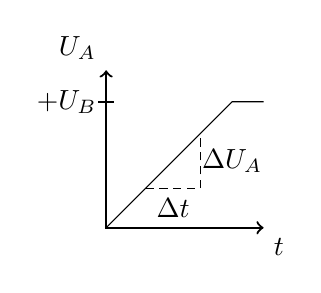
\begin{tikzpicture}
        \draw[thick,->] (-0.015,0) -- (2,0) node[anchor=north west] {$t$};
        \draw[thick,->] (0,0) -- (0,2) node[anchor=south east] {$U_{A}$};
        \draw (0,0) -- (1.6,1.6) -- (2,1.6);
        \draw[thick] (-0.1,1.6) -- (0.1,1.6);
        \draw (0,1.6) node[anchor=east] {$+U_B$};
        
        \draw[densely dashed] (0.5,0.5) -- (1.2,0.5) -- ++(0,0.7);  % Steigungsdreieck Linien
            \node at (1.6,0.85) {$\Delta U_A$};
            \node at (0.85,0.25) {$\Delta t$}; 
    \end{tikzpicture}} \\
    \hline
\end{tabular}}}{Schaltung des Beispielproblems mit einer Signalquelle auf der Eingangsseite und einer komplexen Last auf der Ausgangsseite \label{fig:Beispielproblem 1 Folien 2 Abbildung 1}} 
        }
    \end{frame}
    \begin{frame}
        \b{
            \frametitle{Prinzip der Gegenkopplung - Lösung des Beispielproblems (2)}
             \fu{\resizebox{0.8\textwidth}{!}{\begin{tabular}{|m{0.25\textwidth}|m{0.5\textwidth}|m{0.25\textwidth}|}
    \hline
    \begin{circuitikz}[scale=0.8, transform shape]
        \ctikzset{tripoles/en amp/input height=-0.45}
        \draw (0,0) node[en amp](E){};
        \node at ($(E) + (-1.2, 1.5)$) {\textbf{\LARGE A}}; % Label für den ersten OPV
        \draw (E.out) node[circ]{} node[right]{$U_A$};
        \draw (E.-) node[circ]{} node[left]{0V};
        \draw (E.+) node[circ]{} node[left]{1V};
        \draw (E.up) -- ++(0,0.5) node[anchor=south]{$+U_B$} node[circ] {};
        \draw (E.down) -- ++(0,-0.5) node[anchor=north]{$-U_B$} node[circ] {};
    \end{circuitikz} &
    \begin{circuitikz}[scale=0.8, transform shape]
        \ctikzset{tripoles/en amp/input height=-0.45}
        \draw (0,0) node[en amp](E){};
        \node at ($(E) + (-1.2, 1.5)$) {\textbf{\LARGE B}}; % Label für den ersten OPV im mittleren Bild
        \draw (E.out) node[circ]{} node[right]{$U_A$};
        \draw (E.-) node[circ]{} node[left]{0V} -- ++(0, -1) to[normal open switch] ++(2.38,0) -- ++(0,1.5);
        \draw (E.+) node[circ]{} node[left]{1V};
    
        \draw (4,0) node[en amp](E2){};
        \node at ($(E2) + (-1.2, 1.5)$) {\textbf{\LARGE C}}; % Label für den zweiten OPV im mittleren Bild
        \draw (E2.out) node[circ]{} node[right]{$U_A$};
        \draw (E2.-) node[circ]{} node[left]{0V} -- ++(0, -1) -- ++(2.38,0) -- ++(0,1.5);
        \draw (E2.+) node[circ]{} node[left]{1V};
    \end{circuitikz}
    \\
    \hline
    \multicolumn{1}{|c|}{
    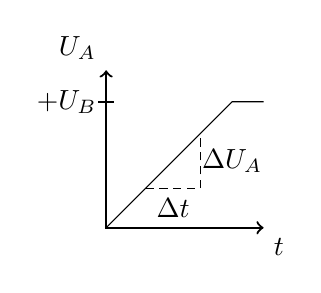
\begin{tikzpicture}
        \draw[thick,->] (-0.015,0) -- (2,0) node[anchor=north west] {$t$};
        \draw[thick,->] (0,0) -- (0,2) node[anchor=south east] {$U_{A}$};
        \draw (0,0) -- (1.6,1.6) -- (2,1.6);
        \draw[thick] (-0.1,1.6) -- (0.1,1.6);
        \draw (0,1.6) node[anchor=east] {$+U_B$};
        
        \draw[densely dashed] (0.5,0.5) -- (1.2,0.5) -- ++(0,0.7);  % Steigungsdreieck Linien
            \node at (1.6,0.85) {$\Delta U_A$};
            \node at (0.85,0.25) {$\Delta t$}; 
    \end{tikzpicture}} &
    \multicolumn{1}{c|}{
    \begin{tikzpicture}
        \draw[thick,->] (1.985,0) -- (4,0) node[anchor=north west] {$t$};
        \draw[thick,->] (2,0) -- (2,2) node[anchor=south east] {$U_{A}$};
        \draw (2,0) -- (3,0.5) -- (4,0.5);
        \draw[thick] (1.9,0.5) -- (2.1,0.5) node[anchor=east] {$1V$};
        \node at (0,1) {Slew rate: $\frac{\Delta U_A}{\Delta t}$};
    \end{tikzpicture}}
    \\
    \hline
    \end{tabular}}}{Schaltung des Beispielproblems mit einer Signalquelle auf der Eingangsseite und einer komplexen Last auf der Ausgangsseite \label{fig:Beispielproblem 1 Folien 2 Abbildung 2}} 
        }
    \end{frame}

%\speech{
% Beispiel 3.1: Teil 1: Entwicklung einer Verstärkerschaltung für Musiksignale.
% Bei der Entwicklung von Hi-Fi-Geräten müssen Verstärker an die Last (also den Lautsprecher) angepasst werden.
% Dazu wird ein Leistungsverstärker (d.h. eine Endstufe) benötigt. Eine solche Endstufe, die geeignet ist, das Signal eines Handys so zu verstärken, dass ein Lautsprecher damit betrieben werden kann soll hier aufgebaut werden.
% Ein vereinfachtes Ersatzschaltbild des Lautsprechers ist durch eine Induktivität mit einem in Reihe geschalteten Widerstand gegeben (siehe Abbildung \ref{fig:Beispielproblem 1}).
% Das Eingangsspannungsniveau ist 1~V und es soll ein 4~$\mathrm{\Omega}$ Lautsprecher betrieben werden (4~$\mathrm{\Omega}$ bedeutet, dass der Lautsprecher bei 1~kHz eine Impedanz von 4~$\Omega$ aufweist).
% Wie groß muss die Spannung am Ausgang des Verstärkers sein, damit der Lautsprecher bei 1~kHz 25 W aufnimmt? Wie kann hier vorgegangen werden, wenn eine Operationsverstärkerschaltung für die Lösung genutzt werden soll?
% Lösung: Zunächst muss dazu die Spannung berechnet werden, die der Verstärker ausgeben soll.
% U A = sqrt(P * R) = sqrt(25 W * 4 $\Omega$) = 10 V
% Wie kann nun mithilfe eines Operationsverstärkers der mit einem ? gekennzeichneten Teil der Schaltung ersetzt werden, um eine notwendige Verstärkung von 10 zu erreichen (siehe Abbildung \ref{fig:Beispielproblem 1})?
%} 

%\speech{
%Abbildung 3.1 zeigt eine Schaltung mit einer Signalquelle auf der Eingangsseite und einer komplexen Last auf der Ausgangsseite.  
%Die Signalquelle liefert eine Wechselspannung mit einer Amplitude von 1 Volt.  
%Das Signal wird an eine unbekannte Schaltung weitergeleitet, die durch ein Fragezeichen gekennzeichnet ist.  
%Diese Schaltung verstärkt oder verändert das Signal und gibt es an die Ausgangslast weiter.  
%
%Die Ausgangslast ist in einem gestrichelten Rechteck markiert und stellt ein Ersatzschaltbild für einen Lautsprecher dar.  
%Diese Last besteht aus einem Widerstand von 2 Ohm in Reihe mit einer Induktivität von 100 Millihenry.  
%Die Induktivität beeinflusst das Verhalten der Last in Abhängigkeit von der Frequenz des Eingangssignals.  
%
%Die Aufgabe besteht darin, den Verstärkungsfaktor der unbekannten Schaltung zu bestimmen.  
%Der Verstärkungsfaktor ist definiert als das Verhältnis der Ausgangsspannung U A zur Eingangsspannung U E.  
%Mathematisch ausgedrückt als V gleich U A geteilt durch U E.  
%
%Um den Verstärkungsfaktor zu berechnen, müssen die Eigenschaften der unbekannten Schaltung sowie die Auswirkungen der komplexen Last berücksichtigt werden.  
%}



\begin{frame}
    \s{\pagebreak
        Wie aus vorherigen Kapiteln bekannt ist, besitzen Operationsverstärker einen invertierenden und einen nicht-invertierenden Eingang. Existiert zwischen diesen beiden Eingängen eine Spannungsdifferenz, so verstärkt der Operationsverstärker diese Differenz um ein Vielfaches, bis die Spannung die maximale Ausgangsspannung des Operationsverstärkers erreicht (siehe A in Abbildung \ref{fig: Verschaltung Verstaerker}).
    Die Slew-Rate (zu deutsch: Anstiegsrate) gibt an, wie schnell dieser Anstieg geschehen kann. Wird die Ausgangsspannung nicht auf den Eingang zurückgeführt, steigt die Ausgangspannung, bis das Niveau der Versorgungsspannung erreicht wird. Eine solche Beschaltung des Verstärkers wird als Komperatorschaltung bezeichet.

    Dieses Verhalten ist für die meisten Anwendungen bei denen der Eingangsspannungssignal mit geringer Amplitude verstärkt werden soll, nicht erwünscht. 
    Stattdessen werden Operationsverstärker meistens in der sogenannten Gegenkopplung (B) betrieben, bei der der Ausgang auf den invertierenden Eingang zurückgeführt wird. 
    Der in (B) eingezeichnete Schalter sei zunächst geöffnet und der Operationsverstärker werde nicht mit Spannung versorgt. Zum Zeitpunkt 0 s wird der Schalter geschlossen und die Versorgungsspannung des Verstärkers eingeschaltet, wodurch die Rückführung des Ausgangssignals $U_{\textnormal{A}}$ aktiv wird (C). 
    Durch die Rückkopplung des Ausgangssignal wird so erreicht, dass die Spannung am invertierenden Eingang auf das Spannungsniveau der Ausgangsspannung angeglichen wird. 
    Die in (C) dargestellte Verstärkerschaltung hat die Verstärkung 1 und wird als Impedanzwandler bezeichnet, da der Verstärker in dieser Schaltungsart aufgrund seiner hohen Eingangsimpedanz verwendet werden kann, um eine Schaltung mit hochohmigem Eingang zu realisieren (dies ist beispielsweise bei Messschaltungen für Spannungsmessungen notwendig). 
    Für die Lösung des Anwendungsproblems ist diese Schaltung allerdings noch nicht geeignet, da eine Verstärkung von 5 gefordert ist. 
    Um diese zu erreichen werden in die Verstärkerschaltung nun zusätzlich Widerstände eingebaut (wie in (D) dargestellt ist)\footnote{Es lässt sich feststellen, dass sich für $R_2 = 0$ und $R_1 = \infty$ wieder die Schaltung des Impedanzwandlers ergibt. Der Impedanzwandler ist also ein Spezialfall des nicht-invertierenden Verstärkers.}.      
    }
    \b{\frametitle{Prinzip der Gegenkopplung - Lösung des Beispielproblems (2)}}
    \fu{
        \resizebox{\textwidth}{!}{\begin{tabular}{|m{0.25\textwidth}|m{0.45\textwidth}|m{0.3\textwidth}|}
    \hline
    \begin{circuitikz}[scale=0.8, transform shape]
        \ctikzset{tripoles/en amp/input height=-0.45}
        \draw (0,0) node[en amp](E){};
        \node at ($(E) + (-1.2, 1.5)$) {\textbf{\LARGE A}}; % Label für den ersten OPV
        \draw (E.out) node[circ]{} node[right]{$U_A$};
        \draw (E.-) node[circ]{} node[left]{0V};
        \draw (E.+) node[circ]{} node[left]{1V};
        \draw (E.up) -- ++(0,0.5) node[anchor=south]{$+U_B$} node[circ] {};
        \draw (E.down) -- ++(0,-0.5) node[anchor=north]{$-U_B$} node[circ] {};

    \end{circuitikz} &
    \begin{circuitikz}[scale=0.8, transform shape]
        \ctikzset{tripoles/en amp/input height=-0.45}
        \draw (0,0) node[en amp](E){};
        \node at ($(E) + (-1.2, 1.5)$) {\textbf{\LARGE B}}; % Label für den ersten OPV im mittleren Bild
        \draw (E.out) node[circ]{} node[right]{$U_A$};
        \draw (E.-) node[circ]{} node[left]{0V} -- ++(0, -1) to[normal open switch] ++(2.38,0) -- ++(0,1.5);
        \draw (E.+) node[circ]{} node[left]{1V};
    
        \draw (4,0) node[en amp](E2){};
        \node at ($(E2) + (-1.2, 1.5)$) {\textbf{\LARGE C}}; % Label für den zweiten OPV im mittleren Bild
        \draw (E2.out) node[circ]{} node[right]{$U_A$};
        \draw (E2.-) node[circ]{} node[left]{0V} -- ++(0, -1) -- ++(2.38,0) -- ++(0,1.5);
        \draw (E2.+) node[circ]{} node[left]{1V};
    \end{circuitikz} &
    \begin{circuitikz}[scale=0.8, transform shape]
        \ctikzset{tripoles/en amp/input height=-0.45,
        }
        \draw (0,0) node[en amp](E){};
        \node at ($(E) + (-1.2, 1.5)$) {\textbf{\LARGE D}}; % Label für den OPV im dritten Bild
        \draw (E.out) node[circ]{} -- ++(0.2,0) node[ocirc, right]{};
        \draw (E.-) -- ++(0, -1.3) node[circ] {} to[R, l=$R_2$] ++(2.38,0) -- ++(0,1.8);
        \draw (E.-) -- ++(0, -1.6) to[R, l_=$R_1$] ++(0, -1.2) -- ++(0,-0.2) -- ++(-0.2, 0) -- ++(0.4,0);
        \draw (E.+) node[circ]{} node[left]{};     
       
        % Spannungspfeil
        \draw[-{Triangle[width=3pt,length=4pt]}, color=spannung] ($(E.+) + (0, -0.1)$) -- ($(E.-) + (0, 0.1)$) node[midway, xshift=-30] {$U_{\text{Diff}}=0\,\text{V}$};
        \draw[-{Triangle[width=3pt,length=4pt]}, color=spannung] ($(E.out) + (0.26, -0.1)$) -- ($(E.out) + (0.26, -3.45)$) node[midway, xshift=10] {$U_A$};
        \draw[black] ($(E.out) + (0.26, -3.5)$) -- ++(-0.2, 0) -- ++(0.4,0);
        \draw[-{Triangle[width=3pt,length=4pt]}, color=spannung] (0.7,-2.1)-- ++(-1.5,0) node[midway, yshift=-10] {$U_{R2}$};
        \draw[-{Triangle[width=3pt,length=4pt]}, color=spannung] (-0.9,-2)-- ++(0,-1.5) node[midway, xshift=10] {$U_{R1}$};


        
        \node[red] at (0.9,-1.8) {\tikz \draw[red, -{Triangle[width=3pt,length=4pt]}] (0,0) -- (-0.01,0);};
        \node[above, color=red] at (0.9,-1.8)  {$I_{R2}$};

        \node[red] at ($(E.-)+(0,-1.5)$) {\tikz \draw[red, -{Triangle[width=3pt,length=4pt]}] (0,0) -- (0,-0.01);};
        \node[left, color=red] at ($(E.-)+(0,-1.4)$)  {$I_{R1}$};
    \end{circuitikz}
    \\
    \hline
    \multicolumn{1}{|c|}{
    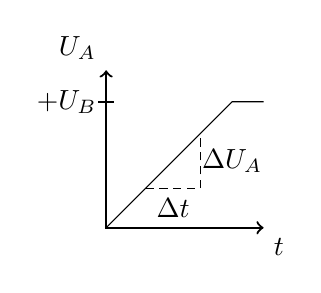
\begin{tikzpicture}
        \draw[thick,->] (-0.015,0) -- (2,0) node[anchor=north west] {$t$};
        \draw[thick,->] (0,0) -- (0,2) node[anchor=south east] {$U_{A}$};
        \draw (0,0) -- (1.6,1.6) -- (2,1.6);
        \draw[thick] (-0.1,1.6) -- (0.1,1.6);
        \draw (0,1.6) node[anchor=east] {$+U_B$};
        
        \draw[densely dashed] (0.5,0.5) -- (1.2,0.5) -- ++(0,0.7);  % Steigungsdreieck Linien
            \node at (1.6,0.85) {$\Delta U_A$};
            \node at (0.85,0.25) {$\Delta t$}; 
    \end{tikzpicture}} &
    \multicolumn{1}{c|}{
    \begin{tikzpicture}
        \draw[thick,->] (1.985,0) -- (4,0) node[anchor=north west] {$t$};
        \draw[thick,->] (2,0) -- (2,2) node[anchor=south east] {$U_{A}$};
        \draw (2,0) -- (3,0.5) -- (4,0.5);
        \draw[thick] (1.9,0.5) -- (2.1,0.5) node[anchor=east] {$1V$};
        \node at (0,1) {Slew rate: $\frac{\Delta U_A}{\Delta t}$};
    \end{tikzpicture}} &
    \multicolumn{1}{c|}{
    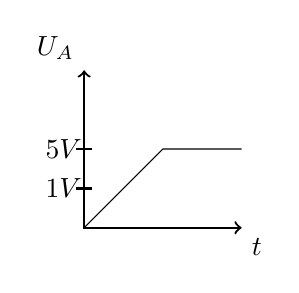
\begin{tikzpicture}
        \draw[thick,->] (-0.015,0) -- (2,0) node[anchor=north west] {$t$};
        \draw[thick,->] (0,0) -- (0,2) node[anchor=south east] {$U_{A}$};
        \draw (0,0) -- (1,1) -- (2,1);
        \draw[thick] (-0.1,1) -- (0.1,1) node[anchor=east] {$5V$};
        \draw[thick] (-0.1,0.5) -- (0.1,0.5) node[anchor=east] {$1V$};
    \end{tikzpicture}} \\
    \hline
    \end{tabular}}
        }{Verschaltung eines Verstärkers als Komperator (A), Impedanzwandler (C) und nicht-invertierender Verstärker (D)
        \label{fig: Verschaltung Verstaerker}}       
\end{frame}

%\speech {
%    Wie aus vorherigen Kapiteln bekannt ist, besitzen Operationsverstärker einen invertierenden und einen nicht-invertierenden Eingang. Existiert zwischen diesen beiden Eingängen eine Spannungsdifferenz, so verstärkt der Operationsverstärker diese Differenz um ein Vielfaches, bis die Spannung die maximale Ausgangsspannung des Operationsverstärkers erreicht (siehe A in Abbildung \ref{fig: Verschaltung Verstaerker}).
%    Die Slew-Rate (zu deutsch: Anstiegsrate) gibt an, wie schnell dieser Anstieg geschehen kann. Wird die Ausgangsspannung nicht auf den Eingang zurückgeführt, steigt die Ausgangspannung, bis das Niveau der Versorgungsspannung erreicht wird. Eine solche Beschaltung des Verstärkers wird als Komperatorschaltung bezeichet.
% Dieses Verhalten ist für die meisten Anwendungen bei denen der Eingangsspannungssignal mit geringer Amplitude verstärkt werden soll, nicht erwünscht.
% Stattdessen werden Operationsverstärker meistens in der sogenannten Gegenkopplung (B) betrieben, bei der der Ausgang auf den invertierenden Eingang zurückgeführt wird.
% Der in (B) eingezeichnete Schalter sei zunächst geöffnet und der Operationsverstärker werde nicht mit Spannung versorgt. Zum Zeitpunkt 0 s wird der Schalter geschlossen und die Versorgungsspannung des Verstärkers eingeschaltet, wodurch die Rückführung des Ausgangssignals $U_{\textnormal{A}}$ aktiv wird (C).
% Durch die Rückkopplung des Ausgangssignal wird so erreicht, dass die Spannung am invertierenden Eingang auf das Spannungsniveau der Ausgangsspannung angeglichen wird.
% Die in (C) dargestellte Verstärkerschaltung hat die Verstärkung 1 und wird als Impedanzwandler bezeichnet, da der Verstärker in dieser Schaltungsart aufgrund seiner hohen Eingangsimpedanz verwendet werden kann, um eine Schaltung mit hochohmigem Eingang zu realisieren (dies ist beispielsweise bei Messschaltungen für Spannungsmessungen notwendig).
% Für die Lösung des Anwendungsproblems ist diese Schaltung allerdings noch nicht geeignet, da eine Verstärkung von 5 gefordert ist.
% Um diese zu erreichen werden in die Verstärkerschaltung nun zusätzlich Widerstände eingebaut (wie in (D) dargestellt ist)\footnote{Es lässt sich feststellen, dass sich für $R_2 = 0$ und $R_1 = \infty$ wieder die Schaltung des Impedanzwandlers ergibt. Der Impedanzwandler ist also ein Spezialfall des nicht-invertierenden Verstärkers.}.
%}
%\speech{
%Abbildung 3.2 zeigt verschiedene Verschaltungen eines Operationsverstärkers und deren zugehörige Ausgangsverläufe.  
%Es sind vier verschiedene Konfigurationen dargestellt:  
%Ein Komparator, zwei Varianten eines Impedanzwandlers und ein nichtinvertierender Verstärker.  
%
%Im oberen Bereich der Abbildung sind die jeweiligen Schaltungen zu sehen.  
%Im unteren Bereich sind die entsprechenden Ausgangsdiagramme dargestellt, die den zeitlichen Verlauf der Ausgangsspannung U A zeigen.  
%
%Schaltung A zeigt einen Operationsverstärker als Komparator.  
%Der nichtinvertierende Eingang erhält eine konstante Spannung von 1 Volt.  
%Der invertierende Eingang ist auf 0 Volt gelegt.  
%Da die Eingangsspannung am nichtinvertierenden Eingang größer ist, springt die Ausgangsspannung auf den maximalen positiven Wert.  
%Das untere Diagramm zeigt den Ausgangsverlauf als sprunghafte Änderung.  
%
%Schaltung B und C zeigen einen Operationsverstärker als Impedanzwandler, auch Unity-Gain-Buffer genannt.  
%Hierbei wird die Eingangsspannung direkt am nichtinvertierenden Eingang angelegt.  
%Der Ausgang ist mit dem invertierenden Eingang verbunden, sodass eine Verstärkung von Eins entsteht.  
%Das untere Diagramm zeigt, dass die Ausgangsspannung genau der Eingangsspannung folgt.  
%
%Schaltung D zeigt einen nichtinvertierenden Verstärker.  
%Ein Spannungsteiler aus den Widerständen R1 und R2 bestimmt die Verstärkung.  
%Die Ausgangsspannung U A ist größer als die Eingangsspannung.  
%Das untere Diagramm zeigt eine Verstärkung des Signals, wobei die Ausgangsspannung von 1 Volt auf 5 Volt ansteigt.  
%
%Die Abbildung zeigt, wie sich unterschiedliche Verschaltungen auf die Ausgangsspannung auswirken.  
%}

\begin{frame}
    \s{
    \begin{bsp}{Teil 2: Entwicklung einer Verstärkerschaltung für Musiksignale}{Beispiel Verstaerkung 2}
        Im letzten Schritt muss ermittelt werden, wie die Widerstände in (D) gewählt werden müssen, damit sich eine Verstärkung von 5 ergibt. Dazu müssen zunächst die Maschengleichungen aufgestellt werden.
        Eine wichtige Annahme zur Aufstellung dieser Maschengleichung ist, dass davon ausgegangen wird, dass der Verstärker durch die Rückkopplung des Ausgangsignal die beiden Eingangssignale angleicht. 
        Hier darf also geschrieben werden \glqq Annahme: $U_{\textnormal{dif}}~=~0$~V\grqq{}. 
        Somit ergibt sich für den invertierenden Eingang $U_{\textnormal{E-}}~=~1$~V.
        Da weiterhin davon ausgegangen wird, dass kein Strom in die Eingänge hineinfließt gilt $I_{\textnormal{R1}}~=~I_{\textnormal{R2}}$.
        Die Maschengleichung lautet auf Grundlage dieser Annahmen
        \begin{equation}
            U_{\textnormal{A}} = U_{\textnormal{R1}} + U_{\textnormal{R2}} = U_{\textnormal{E}} + I_{\textnormal{R2}} \cdot R_{\textnormal{2}} = U_{\textnormal{E}} + \frac{U_{\textnormal{E}}}{R_{\textnormal{1}}} \cdot R_{\textnormal{2}} 
        \end{equation}

        Dadurch ergibt sich das Ein-Ausgangsverhalten im zeitbereich zu folgendem Ausdruck.
        \begin{equation}
            \frac{U_{\textnormal{A}}}{U_{\textnormal{E}}} = \underbrace{(1+\frac{R_2}{R_1})}_{V}
        \end{equation}
        

        Wird diese Gleichung nach $R_2/R_1$ gelöst, ergibt sich das Verhältnis der Widerstände für das oben beschriebene 
        Problem zu $R_2/R_1 = 9$. Die Widerstände sollten hier nicht zu groß gewählt werden, da dann der Ausgleichsstrom zwischen
        Ausgang und Eingang zu klein werden könnte. Das kann zu einem starken Rauschen am Verstärkerausgang führen. Übliche Widerstandswerte sind in der Regel den Beispielschaltungen des Datenblattes eines
        Operationsverstärkers zu entnehmen. In diesem Fall könnte z.B. $R_2=9~\textnormal{k}\Omega$ und $R_1=1~\textnormal{k}\Omega$ gewählt werden.
    \end{bsp} 

%\speech{1}{
%Beispiel 3.2: Teil 2: Entwicklung einer Verstärkerschaltung für Musiksignale.
%Im letzten Schritt muss ermittelt werden, wie die Widerstände in (D) gewählt werden müssen, damit sich eine Verstärkung von 5 ergibt. Dazu müssen zunächst die Maschengleichungen aufgestellt werden.
%Eine wichtige Annahme zur Aufstellung dieser Maschengleichung ist, dass davon ausgegangen wird, dass der Verstärker durch die Rückkopplung des Ausgangsignal die beiden Eingangssignale angleicht.
%Hier darf also geschrieben werden \glqq Annahme: $U_{\textnormal{dif}}~=~0$~V\grqq{}.
%Somit ergibt sich für den invertierenden Eingang $U_{\textnormal{E-}}~=~1$~V.
%Da weiterhin davon ausgegangen wird, dass kein Strom in die Eingänge hineinfließt gilt $I_{\textnormal{R1}}~=~I_{\textnormal{R2}}$.
%Die Maschengleichung lautet auf Grundlage dieser Annahmen
%\begin{equation}
%    U_{\textnormal{A}} = U_{\textnormal{R1}} + U_{\textnormal{R2}} = U_{\textnormal{E}} + I_{\textnormal{R2}} \cdot R_{\textnormal{2}} = U_{\textnormal{E}} + \frac{U_{\textnormal{E}}}{R_{\textnormal{1}}} \cdot R_{\textnormal{2}}
%\end{equation}
%Wird diese Gleichung nach $R_2/R_1$ gelöst, ergibt sich das Verhältnis der Widerstände für das oben beschriebene 
%Problem zu $R_2/R_1 = 9$. Die Widerstände sollten hier nicht zu groß gewählt werden, da dann der Ausgleichsstrom zwischen
%Ausgang und Eingang zu klein werden könnte. Das kann zu einem starken Rauschen am Verstärkerausgang führen. Übliche Widerstandswerte sind in der Regel den Beispielschaltungen des Datenblattes eines
%Operationsverstärkers zu entnehmen. In diesem Fall könnte z.B. $R_2=9~\textnormal{k}\Omega$ und $R_1=1~\textnormal{k}\Omega$ gewählt werden.
%}
        \par
        Ähnnlich wie für die oben dargestellte Schaltung lassen sich auch für alle weiteren Operationsverstärkerschaltungen Übertragungsfunktionen herleiten. Das soll hier allerdings nicht gezeigt werden.
        Weitere Übertragungsfuktionen für einige ausgewählte Operationsverstärkergrundschaltungen können Tabelle \ref{tab:Grundschaltungen} entnommen werden. 
        In dieser Tabelle sind die die Schaltungen, die Bodediagramme mit Phasengang (rot) und Amplitudengang (blau) und die Übertragungsfunktionen angegeben. 
        Nachdem nun die Beschaltung von Verstärkern vorgestellt wurde, soll im Folgenden Kapitel nun noch eine wichtige Eigenschaft von Verstärkerschaltungen thematisiert werden, die sich aus den genutzen Verstärkerbausteinen und der äußeren Verschaltung ergibt: Die Stabilität der Verstärkerschaltung.
        
%\speech {1}{
% Ähnlich wie für die oben dargestellte Schaltung lassen sich auch für alle weiteren Operationsverstärkerschaltungen Übertragungsfunktionen herleiten. Das soll hier allerdings nicht gezeigt werden.
%    Weitere Übertragungsfuktionen für einige ausgewählte Operationsverstärkergrundschaltungen können Tabelle \ref{tab:Grundschaltungen} entnommen werden.
%    In dieser Tabelle sind die die Schaltungen, die Bodediagramme mit Phasengang (rot) und Amplitudengang (blau) und die Übertragungsfunktionen angegeben.
%    Nachdem nun die Beschaltung von Verstärkern vorgestellt wurde, soll im Folgenden Kapitel nun noch eine wichtige Eigenschaft von Verstärkerschaltungen thematisiert werden, die sich aus den genutzen Verstärkerbausteinen und der äußeren Verschaltung ergibt: Die Stabilität der Verstärkerschaltung.   
%}
        
%\speech{
%Tabelle 3.1 zeigt verschiedene Grundschaltungen mit Operationsverstärkern.  
%Die Tabelle ist in drei Spalten unterteilt.  
%Die erste Spalte zeigt die Schaltung, die zweite Spalte enthält den Frequenzgang und die Gleichung,  
%und die dritte Spalte gibt eine Erklärung mit den wichtigsten Eigenschaften.  
%
%Erste Zeile: Nichtinvertierender Verstärker.  
%Die Ausgangsspannung ist phasengleich mit der Eingangsspannung.  
%Die Verstärkung ist eins plus das Verhältnis von R2 zu R1.  
%Der Verstärker hat einen sehr hohen Eingangswiderstand und einen niedrigen Ausgangswiderstand.  
%Anwendungsbeispiel ist ein Impedanzwandler.  
%
%Zweite Zeile: Invertierender Verstärker.  
%Die Ausgangsspannung ist um 180 Grad phasenverschoben zur Eingangsspannung.  
%Die Verstärkung ist das Verhältnis von R2 zu R1.  
%Der Widerstand R1 bestimmt den Eingangswiderstand.  
%Anwendungsbeispiel ist ein aktiver Spannungsteiler für hohe Spannungen.  
%
%Dritte Zeile: Komparator.  
%Die Ausgangsspannung ist entweder hoch oder niedrig, je nach Vergleich der Eingänge.  
%Wenn die nichtinvertierende Spannung größer ist als die invertierende Spannung,  
%geht die Ausgangsspannung auf den oberen Versorgungswert.  
%Andernfalls geht sie auf den unteren Versorgungswert.  
%Wird verwendet in Zweipunktreglern und Analog-Digital-Wandlern.  
%
%Vierte Zeile: Summierer.  
%Der Summierer basiert auf einem invertierenden Verstärker.  
%Die Ausgangsspannung ist eine gewichtete Summe mehrerer Eingangsspannungen.  
%Wird verwendet in Analogrechnern und zur Mischung von Signalen.  
%
%Fünfte Zeile: Subtrahierer.  
%Diese Schaltung bildet die Differenz zwischen zwei Eingangsspannungen.  
%Wenn alle Widerstände gleich sind, entspricht die Ausgangsspannung genau der Differenz der Eingänge.  
%Diese Schaltung wird als Differenzverstärker verwendet.  
%
%Sechste Zeile: Integrierer.  
%Der Integrierer summiert die Eingangsspannung über die Zeit.  
%Die Ausgangsspannung entspricht dem negativen Integral des Eingangssignals.  
%Wird als aktiver Tiefpassfilter verwendet.  
%
%Siebte Zeile: Differenzierer.  
%Der Differenzierer bildet die Ableitung des Eingangssignals.  
%Die Ausgangsspannung ist proportional zur zeitlichen Änderung der Eingangsspannung.  
%Wird als Hochpassfilter eingesetzt, zeigt in der Praxis aber oft ein Bandpassverhalten.  
%
%Diese Tabelle gibt einen Überblick über wichtige Operationsverstärkerschaltungen  
%und ihre typischen Anwendungen in der Signalverarbeitung.  
%}



        \begin{block}{}
            \begin{table}[ht]
    \caption{Ausgewählte Operationsverstärker-Grundschaltungen}
    \label{tab:Grundschaltungen}
    \begin{tabular}{|m{0.24\textwidth}|m{0.405\textwidth}|m{0.33\textwidth}|}
    \hline
    Schaltung & Frequenzgang und Gleichung & Erläuterung und Eigenschaften\\ % Neue Zeile mit Text
    \hline
    \vspace{0.5cm}
    \centering
    \begin{circuitikz}[scale=0.7, transform shape]
    \ctikzset{
         resistors/scale=0.8,              
         tripoles/en amp/height=1.4, % Höhe des OPV             
         tripoles/en amp/width=1.4,   % Breite des OPV
         tripoles/en amp/input height=-0.45
    }
    \vspace{1ex}
    \draw (2,-0.1) node[en amp] (opamp) {}
    (opamp.+) --++ (-0.5,0) node[ocirc, label=left:$U_E$] (eingang) {} 
    (opamp.out) --++ (0.5,0) node[ocirc, label=right:$U_A$] {}
    (opamp.-) -- ++(0, -1.5) to[R, l=$R_1$] ++(0, -1) node[ground] {}
    (opamp.out) node[circ] {} -- ++(0,-1.5) to[R, l=$R_2$] ++(-1.95,0) node[circ] (feedback) {};
\end{circuitikz}

 & \begin{tikzpicture}[scale=1, transform shape]
    \begin{axis}[
    width=4.5cm, % Breite des Graphen
    height=3.5cm, % Höhe des Graphen
    xmin=0, xmax=10,
    ymin=0, ymax=120,
    axis lines=left,
    axis on top=true,
    domain=0:10,
    xtick=\empty,
    ytick=\empty,
    ylabel style={rotate=270, anchor=east, yshift=1cm}, % Position der Beschriftung oben links, horizontal
     ylabel={\it V}, % Hier die gewünschte Beschriftung einfügen
    xlabel={f[Hz]},
    clip mode=individual % Verhindert das Abschneiden von Elementen
    ]
    \path[draw=none] (axis cs:-4, 0) rectangle (axis cs:16.6,120);
    
    
    \coordinate (xaxis) at (axis description cs:15.5,0); % Verwendet die relative Positionierung für x-Achse
    
    \addplot+[mark=none, thick, blue] coordinates {(0,80) (10,80)};
    % Adding the left-side label
    \node[anchor=east] at (axis cs:0,80) {$1 + \frac{R_2}{R_1}$};
    \end{axis}
    \begin{axis}[
    width=4.5cm, % Breite des Graphen
    height=3.5cm, % Höhe des Graphen
    xmin=0, xmax=10,
    ymin=-180, ymax=180,
    axis y line*=right,
    axis x line=none,
    ytick=\empty,
    ylabel={$\varphi$},
    ylabel style={rotate=270, anchor=west, yshift=0.8cm},
    clip mode=individual, % Verhindert das Abschneiden von Elementen
    after end axis/.code={
        \draw[->] (axis cs:10,180) -- (axis cs:10,190);
    }
    ]
    \addplot+[mark=none, thick, red] coordinates {(0,0) (10,0)};
    \node[anchor=west] at (axis cs:10,0) {$0^\circ$};
    \end{axis}
    \end{tikzpicture}
\vspace{1ex}
\[
U_{\textnormal{A}} = \left(1+\frac{R_2}{R_1}\right) U_{\textnormal{E}}
\]
    &
    \textbf{Nicht-invertierender Verstärker}
\begin{itemize}
    \item Phasengleiches Ausgangs-\linebreak signal
    \item Sehr hochohmiger Eingangswiderstand
    \item Niederohmiger Ausgangs-\linebreak widerstand
    \item Anwendungen: z.B. Impedanzwandler
\end{itemize} \\
    \hline
    \centering
    \begin{circuitikz}[scale=0.7, transform shape]
    \ctikzset{
          resistors/scale=0.8,              
          tripoles/en amp/height=1.4, % Höhe des OPV             
          tripoles/en amp/width=1.4,   % Breite des OPV
         tripoles/en amp/input height=0.45
     }
     \draw
     (0,0) node[en amp] (opamp) {}
     (opamp.-) to[R, l_=$R_1$, *-] ++(-1.2,0) to[short, o-] ++(0,0) node[left] {$U_E$}
     (opamp.+) -- ++(0,0) node[ground] {}
     (opamp.-) |- ++(0,1) to[R, l=$R_2$] ++(1.9,0) -| (opamp.out)
     (opamp.out) to[short, *-o] ++(0.2,0) node[right] {$U_{A}$};
 \end{circuitikz}
     & 
    \begin{center}
        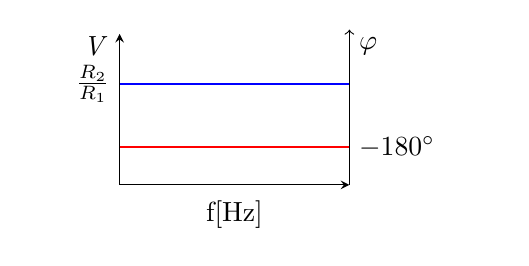
\begin{tikzpicture}[scale=1, transform shape]
    \begin{axis}[
        width=4.5cm, % Breite des Graphen
        height=3.5cm, % Höhe des Graphen
        xmin=0, xmax=10,
        ymin=0, ymax=120,
        axis lines=left,
        axis on top=true,
        domain=0:10,
        xtick=\empty,
        ytick=\empty,
        ylabel style={rotate=270, anchor=east, yshift=0.8cm},
         ylabel={\it V},
        xlabel={f[Hz]},
        clip mode=individual % Verhindert das Abschneiden von Elementen
        ]
        \path[draw=none] (axis cs:-4, 0) rectangle (axis cs:16.6,120);
    
        \addplot+[mark=none, thick, blue] coordinates {(0,80) (10,80)};
        % Adding the left-side label
        \node[anchor=east] at (axis cs:0,80) {$\frac{R_2}{R_1}$};
    \end{axis}
    \begin{axis}[
        width=4.5cm, % Breite des Graphen
        height=3.5cm, % Höhe des Graphen
        xmin=0, xmax=10,
        ymin=-180, ymax=180,
        axis y line*=right,
        axis x line=none,
        ytick=\empty,
        ylabel={$\varphi$},
        ylabel style={rotate=270, anchor=west, yshift=0.8cm},
        clip mode=individual, % Verhindert das Abschneiden von Elementen
        after end axis/.code={
            \draw[->] (axis cs:10,180) -- (axis cs:10,190);
        }
        ]
        \addplot+[mark=none, thick, red] coordinates {(0,-90) (10,-90)};
        \node[anchor=west] at (axis cs:10,-90) {$-180^\circ$};
    \end{axis}
    \end{tikzpicture}
\end{center}
\vspace{1ex}
\[
    U_{\textnormal{A}} = \frac{R_2}{R_1} U_{\textnormal{E}}
\]
    &
    \textbf{Invertierender Verstärker}
\begin{itemize}
    \item -180$^\circ$ Phasenverschiebung zwischen Ein- zu Ausgang
    \item $R_1$ bestimmt den Eingangswiderstand
    \item Niederohmiger Ausgangs-\linebreak widerstand
    \item Anwendungen: \linebreak z.B. Aktiver Spannungsteiler zum Messen hoher Spannungen, wenn $R_1 > R_2$
\end{itemize}
\\ % Zweite Zeile
    \hline
    \centering
    \begin{circuitikz}[scale=0.7, transform shape]
    \ctikzset{
          resistors/scale=0.8,              
          tripoles/en amp/height=1.4, % Höhe des OPV             
          tripoles/en amp/width=1.4,   % Breite des OPV
         tripoles/en amp/input height=0.45
     }
     \draw
     (0,0) node[en amp] (opamp) {}
     (opamp.-)  to[short, o-] ++(0,0) node[left] {$U_{E-}$}
      (opamp.+) to[short, o-] ++(0,0) node[left] {$U_{E+}$}
     (opamp.out) to[short, -o] ++(0,0) node[right] {$U_{A}$};
 \end{circuitikz}
    & 
    \begin{center}
               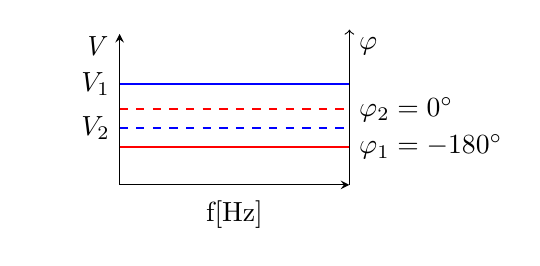
\begin{tikzpicture}[scale=1, transform shape]
    \begin{axis}[
        width=4.5cm, % Breite des Graphen
        height=3.5cm, % Höhe des Graphen
        xmin=0, xmax=10,
        ymin=0, ymax=120,
        axis lines=left,
        axis on top=true,
        domain=0:10,
        xtick=\empty,
        ytick=\empty,
        ylabel style={rotate=270, anchor=east, yshift=0.8cm},
         ylabel={\it V},
        xlabel={f[Hz]},
        clip mode=individual % Verhindert das Abschneiden von Elementen
        ]
        \path[draw=none] (axis cs:-4, 0) rectangle (axis cs:16.6,120);

        \addplot+[mark=none, thick, blue] coordinates {(0,80) (10,80)};
        \addplot+[mark=none, thick, blue, dashed] coordinates {(0,45) (10,45)};
        % Adding the left-side label
        \node[anchor=east] at (axis cs:0,80) {$V_1$};
        \node[anchor=east] at (axis cs:0,45) {$V_2$};
    \end{axis}
    \begin{axis}[
        width=4.5cm, % Breite des Graphen
        height=3.5cm, % Höhe des Graphen
        xmin=0, xmax=10,
        ymin=-180, ymax=180,
        axis y line*=right,
        axis x line=none,
        ytick=\empty,
        ylabel={$\varphi$},
        ylabel style={rotate=270, anchor=west, yshift=0.8cm},
        clip mode=individual, % Verhindert das Abschneiden von Elementen
        after end axis/.code={
            \draw[->] (axis cs:10,180) -- (axis cs:10,190);
        }
        ]
        \addplot+[mark=none, thick, red, dashed] coordinates {(0,0) (10,0)};
        \addplot+[mark=none, thick, red] coordinates {(0,-90) (10,-90)};
        \node[anchor=west] at (axis cs:10,0) {$\varphi_2 = 0^\circ$};
        \node[anchor=west] at (axis cs:10,-90) {$\varphi_1 = -180^\circ$};
    \end{axis}
    \end{tikzpicture}
\[
V_1: U_{\textnormal{E+}} > U_{\textnormal{E-}} \Rightarrow U_{\textnormal{A}} \approx +U_{\textnormal{B}}
\]
\[
V_2: U_{\textnormal{E+}} < U_{\textnormal{E-}} \Rightarrow U_{\textnormal{A}} \approx -U_{\textnormal{B}}
\]
\end{center}
    &\textbf{Komparator}\newline
    Einsatz in Zweipunktreglern und Analog-Digital-Wandlern
\\ % Dritte Zeile
    \hline

    

\centering
\begin{circuitikz}[scale=0.7, transform shape]
    \ctikzset{
        resistors/scale=0.8,              
        tripoles/en amp/height=1.4, % Höhe des OPV             
        tripoles/en amp/width=1.4,   % Breite des OPV
        tripoles/en amp/input height=0.45
    }
    \draw
    (0,0) node[en amp] (opamp) {}
    % R2 mit korrigiertem Strompfeil
    (opamp.-) -- ++(-0.4,0) node[circ] {} to[R, l_=$R_2$] ++(-1.5,0) node[ocirc] (R2left) {}
    % R1 mit korrigiertem Strompfeil
    (opamp.-) -- ++(-0.4,0) --++(0,1) to[R, l_=$R_1$] ++(-1.5,0) node[ocirc] (R1left) {}
    % Erdung
    (opamp.+) -- ++(0,0) node[ground] {}
    % Ausgang
    (opamp.out) to[short, *-o] ++(0,0) node[right] {$U_{A}$}
    % R3 mit Strompfeil
    (opamp.out) -- ++(0,1.5) to[R, l_=$R_3$] ++(-2,0) -- ++(0,-1.05) node[circ] {}
    % Spannungen U_E1 und U_E2 an den Knoten links von R1 und R2
    (R1left) node[left] {$U_{E1}$}
    (R2left) node[left] {$U_{E2}$};
\end{circuitikz}

    &
    \begin{center}
    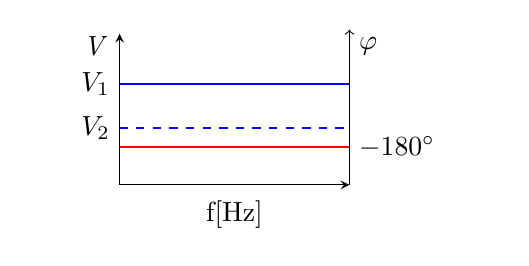
\begin{tikzpicture}[scale=1, transform shape]
    \begin{axis}[
        width=4.5cm, % Breite des Graphen
        height=3.5cm, % Höhe des Graphen
        xmin=0, xmax=10,
        ymin=0, ymax=120,
        axis lines=left,
        axis on top=true,
        domain=0:10,
        xtick=\empty,
        ytick=\empty,
        ylabel style={rotate=270, anchor=east, yshift=0.8cm},
         ylabel={\it V},
        xlabel={f[Hz]},
        clip mode=individual % Verhindert das Abschneiden von Elementen
        ]
        \addplot+[mark=none, thick, blue] coordinates {(0,80) (10,80)};
        \addplot+[mark=none, thick, blue, dashed] coordinates {(0,45) (10,45)};
    
        % Adding the left-side label
        \node[anchor=east] at (axis cs:0,80) {$V_1$};
        \node[anchor=east] at (axis cs:0,45) {$V_2$};
    \end{axis}
    \begin{axis}[
        width=4.5cm, % Breite des Graphen
        height=3.5cm, % Höhe des Graphen
        xmin=0, xmax=10,
        ymin=-180, ymax=180,
        axis y line*=right,
        axis x line=none,
        ytick=\empty,
        ylabel={$\varphi$},
        ylabel style={rotate=270, anchor=west, yshift=0.8cm},
        clip mode=individual, % Verhindert das Abschneiden von Elementen
        after end axis/.code={
            \draw[->] (axis cs:10,180) -- (axis cs:10,190);
        }
        ]
        \path[draw=none] (axis cs:-4, 0) rectangle (axis cs:16.6,120);
        \addplot+[mark=none, thick, red] coordinates {(0,-90) (10,-90)};
        \node[anchor=west] at (axis cs:10,-90) {$-180^\circ$};
    \end{axis}
    \end{tikzpicture}
\end{center}
\vspace{1ex}
\[
\begin{aligned}
    U_{\textnormal{A}} = \underbrace{\frac{R_3} {R_1}}_{V_1} \cdot U_{\textnormal{E1}} + \underbrace{\frac{R_3} {R_2}}_{V_2} \cdot U_{\textnormal{E2}}
\end{aligned}
\]
    & 
    \textbf{Summierer}\newline
    Der Summierer basiert auf dem invertierenden Verstärker und findet Verwendung in Analogrechnern und beim Mischen von Spannungssignalen
    \\ % Vierte Zeile
    \hline
    
    \end{tabular}
\end{table}


\newpage












\begin{table}[ht]
    \begin{tabular}{|m{0.23\textwidth}|m{0.44\textwidth}|m{0.33\textwidth}|}
     \hline 
    Schaltung & Frequenzgang und Gleichung & Erläuterung und Eigenschaften \\ % Neue Zeile mit Text
    \hline
    \begin{circuitikz}[scale=0.7, transform shape]
    \ctikzset{
          resistors/scale=0.8,              
          tripoles/en amp/height=1.4, % Höhe des OPV             
          tripoles/en amp/width=1.4,   % Breite des OPV
         tripoles/en amp/input height=0.45
     }
     \draw
     (0,0) node[en amp] (opamp) {}
     (opamp.-) to[R, l_=$R_1$, o-] ++(-1.2,0) to[short, o-] ++(0,0) node[left] {$U_{E1}$}
     (opamp.+) node[circ] {} to[R,  l_=$R_4$] ++(0,-1.5) node[ground] {}
     (opamp.-) node[circ] {} -- ++(0,1) to[R, l=$R_2$] ++(1.9,0) -| (opamp.out)
     (opamp.out) to[short, *-o] ++(0.2,0) node[right] {$U_{A}$}
     (opamp.+) to[R, l_=$R_3$, *-] ++(-1.2,0) to[short, o-] ++(0,0) node[left] {$U_{E2}$};
 \end{circuitikz}
      &
      \begin{center}
      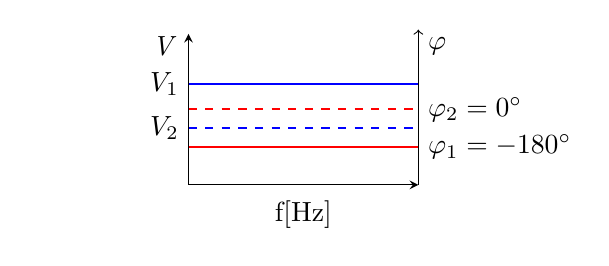
\begin{tikzpicture}[scale=1, transform shape]
    \begin{axis}[
        width=4.5cm, % Breite des Graphen
        height=3.5cm, % Höhe des Graphen
        xmin=0, xmax=10,
        ymin=0, ymax=120,
        axis lines=left,
        axis on top=true,
        domain=0:10,
        xtick=\empty,
        ytick=\empty,
        ylabel style={rotate=270, anchor=east, yshift=0.8cm},
         ylabel={\it V},
        xlabel={f[Hz]},
        clip mode=individual % Verhindert das Abschneiden von Elementen
        ]
        \addplot+[mark=none, thick, blue] coordinates {(0,80) (10,80)};
        \addplot+[mark=none, thick, blue, dashed] coordinates {(0,45) (10,45)};
        % Adding the left-side label
        \node[anchor=east] at (axis cs:0,80) {$V_1$};
        \node[anchor=east] at (axis cs:0,45) {$V_2$};
    \end{axis}
    \begin{axis}[
        width=4.5cm, % Breite des Graphen
        height=3.5cm, % Höhe des Graphen
        xmin=0, xmax=10,
        ymin=-180, ymax=180,
        axis y line*=right,
        axis x line=none,
        ytick=\empty,
        ylabel={$\varphi$},
        ylabel style={rotate=270, anchor=west, yshift=0.8cm},
        clip mode=individual, % Verhindert das Abschneiden von Elementen
        after end axis/.code={
            \draw[->] (axis cs:10,180) -- (axis cs:10,190);
        }
        ]
        \addplot+[mark=none, thick, red, dashed] coordinates {(0,0) (10,0)};
        \addplot+[mark=none, thick, red] coordinates {(0,-90) (10,-90)};
        \node[anchor=west] at (axis cs:10,0) {$\varphi_2 = 0^\circ$};
        \node[anchor=west] at (axis cs:10,-90) {$\varphi_1 = -180^\circ$};
   
   
        \path[draw=none] (axis cs:-7, 0) rectangle (axis cs:16.6,120);
   
   
   
   
    \end{axis}
    \end{tikzpicture}
 \end{center}
 \vspace{1ex}
 \[
 \begin{aligned}
    {U_A} = {U_{{\textnormal{E2}}}} \cdot \underbrace{ \frac{R_1 + R_2}{R_1} \cdot \frac{R_4}{R_3 + R_4}}_{V_2} - U_{\textnormal{E1}} \cdot \underbrace{\frac{R_2}{R_1}}_{V_1}
\end{aligned}
 \]
     &
     \textbf{Subtrahierer}\newline
     Wenn alle Widerstände gleich groß sind, wird die Differenz der Signale $U_{E1}$ und $U_{E2}$ gebildet, weswegen diese Schaltung als Differenzverstärker bezeichnet wird
 \\ % Fünfte Zeile
     \hline

    \begin{circuitikz}[scale=0.7, transform shape]
    \ctikzset{
          resistors/scale=0.8,              
          tripoles/en amp/height=1.4, % Höhe des OPV             
          tripoles/en amp/width=1.4,   % Breite des OPV
         capacitors/scale=0.5,
         tripoles/en amp/input height=0.45
     }
     \vspace{1ex}
     \draw (2,0) node[en amp] (opamp) {}
     (opamp.+) --++ (-0.5,0) node[ground] {} 
     (opamp.out) --++ (0.2,0) node[ocirc, label=right:$U_A$] {}
     (opamp.-) -- ++(0, 0) to[R, l_=$R_1$] ++(-1.2, 0) node[ocirc, label=left:$U_E$] {}
     
     (opamp.out) node[circ] {} -- ++(0,1.5) to[C, l_=$C_1$, *-] ++(-1.9,0) node[circ]{}
     (opamp.out) node[circ] {} -- ++(0,2.8) to[R, l_=$R_2$] ++(-1.9,0) -- ++(0, -2.35) node[circ] {};
     \end{circuitikz}
     & 
     \begin{center}
    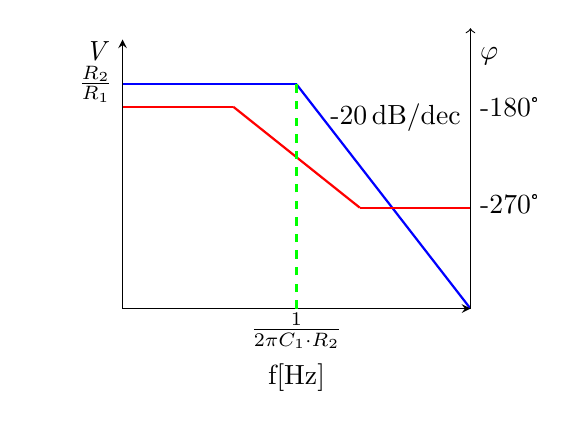
\begin{tikzpicture}[scale=1, transform shape]
    \begin{axis}[
       width=6cm, % Breite des Graphen
       height=5cm, % Höhe des Graphen
        xmin=0, xmax=11,
        ymin=0, ymax=1.2,
        axis lines=center,
        axis on top=true,
        domain=0:10,
        xtick=\empty,
        ytick=\empty,
        ylabel style={xshift=-0.6cm, yshift=0.1cm },
       ylabel={\it V},
       xlabel style={yshift=-0.4cm },
        xlabel={f[Hz]},
        clip mode=individual, % Verhindert das Abschneiden von Elementen
        xlabel style={at={(axis description cs:0.5,-0.05)},anchor=north}
        ]

        \path[draw=none] (axis cs:-3, 0) rectangle (axis cs:13,1);



        \addplot+[mark=none, thick, blue] coordinates {(0,1) (5.5,1)};
        \addplot+[mark=none, thick, blue] coordinates {(5.5,1) (11,0)};
        \node[anchor=east] at (axis cs:0,1) {$\frac{R_2}{R_1}$};
       \node[anchor=east] at (axis cs:11,0.85) {-20\,\text{dB/dec}};
    \end{axis}
    
    \begin{axis}[
       width=6cm, % Breite des Graphen
       height=5cm, % Höhe des Graphen
       xmin=0, xmax=11,
       ymin=0, ymax=240, 
       axis y line*=right,
       axis x line=none,
       ylabel={$\varphi$},
       ylabel style={rotate=270, anchor=west, yshift=1.5cm},
       xtick=\empty,
       ytick=\empty,
       clip mode=individual, % Verhindert das Abschneiden von Elementen
       after end axis/.code={
           \draw[->] (axis cs:11,240) -- (axis cs:11,250);
       }
        ]
        \addplot+[mark=none, thick, red] coordinates {(0,180) (3.5,180)};
        \addplot+[mark=none, thick, red] coordinates {(3.5,180) (7.5,90)};
        \addplot+[mark=none, thick, red] coordinates {(7.5,90) (11,90)};
        \addplot+[mark=none,dashed, thick, green] coordinates {(5.5,0) (5.5,200)};
        \node[] at (axis cs:5.5,-20) {$\frac{1}{2 \pi C_1 \cdot R_2}$};
        \node[anchor=west] at (axis cs:11,180) {-180°};
        \node[anchor=west] at (axis cs:11,93) {-270°};
    \end{axis}
    \end{tikzpicture}
     \[
     U_A(t) = - \frac{R_2}{R_1} U_{\textnormal{E}}(t) - \int_0^t \frac{U_{\textnormal{E}}(t)}{R_1 C_1} \, dt
     \]
     \end{center} 
     &
    \textbf{Integrierer/Integrator}\newline
    \begin{itemize}
        \item Nimmt eine Integration des Eingangssignals vor
        \item Wird als aktives Tiefpassfilter verwendet
    \end{itemize}
      \\ 
      \hline
    \begin{circuitikz}[scale=0.7, transform shape]
    \ctikzset{
          resistors/scale=0.8,              
          tripoles/en amp/height=1.4, % Höhe des OPV             
          tripoles/en amp/width=1.4,   % Breite des OPV
         capacitors/scale=0.5,
         tripoles/en amp/input height=0.45
     }
     \draw (2,0) node[en amp] (opamp) {}
     (opamp.+) --++ (-0.5,0) node[ground] {} 
     (opamp.out) --++ (0.2,0) node[ocirc, label=right:$U_A$] {}
     (opamp.-) -- ++(0, 0) to[C, l_=$C_2$] ++(-0.5, 0) to[R, l_=$R_1$] ++(-1.2,0) node[ocirc, label=left:$U_E$] {}
     (opamp.out) node[circ] {} -- ++(0,1.5) to[C, l_=$C_1$, *-] ++(-1.9,0) node[circ]{}
     (opamp.out) node[circ] {} -- ++(0,2.8) to[R, l_=$R_2$] ++(-1.9,0) -- ++(0, -2.35) node[circ] {};
  
 \end{circuitikz}
    &
    \begin{center}
    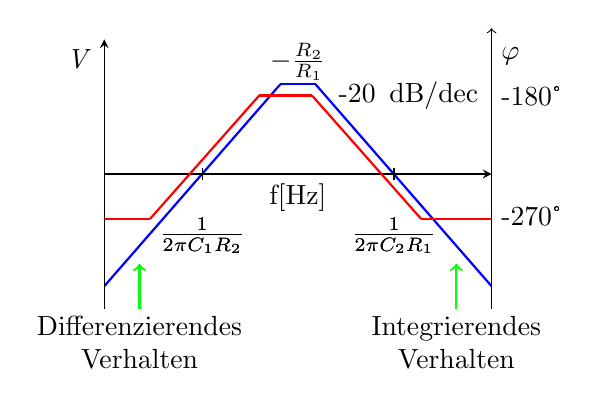
\begin{tikzpicture}[scale=1, transform shape]
    \begin{axis}[
        width=6.5cm, % Breite des Graphen
        height=5cm, % Höhe des Graphen
        xmin=0, xmax=11,
        ymin=-1.2, ymax=1.2,
        axis lines=center,
        axis on top=true,
        domain=0:10,
        clip mode=individual, % Verhindert das Abschneiden von Elementen
        xtick=\empty,
        ytick=\empty,
        ylabel style={xshift=-0.6cm},
        ylabel={\it V},
        xlabel={f[Hz]},
        xlabel style={at={(axis description cs:0.5,0.5)},anchor=north}
        ]
        \path[draw=none] (axis cs:-2, 0) rectangle (axis cs:13,1); \path[draw=none] (axis cs:-2, 0) rectangle (axis cs:13,1);


        \addplot+[mark=none, thick, blue] coordinates {(0,-1) (5,0.8)};
        \addplot+[mark=none, thick, blue] coordinates {(5,0.8) (6,0.8)};
        \addplot+[mark=none, thick, blue] coordinates {(6,0.8) (11,-1)};
        \node[anchor=north] at (axis cs:5.5,1.25) {$-\frac{R_2}{R_1}$};
        \addplot+[only marks, mark=|, black] coordinates {(2.78,0)} node[anchor=south] at (axis cs:2.78,-0.8) {$\frac{1}{2 \pi C_1 R_2}$};
        \addplot+[only marks, mark=|, black] coordinates {(8.23,0)} node[anchor=south] at (axis cs:8.23,-0.8) {$\frac{1}{2\pi C_2 R_1}$};
        \node[anchor=east] at (axis cs:10.9,0.7) {-20\, \text{dB/dec}};
        \addplot+[only marks, mark=|, black] coordinates {(2.78,0)} node[anchor=south] at (axis cs:2.78,-0.8) {$\frac{1}{2 \pi C_1 R_2}$};
        \addplot+[only marks, mark=|, black] coordinates {(8.23,0)} node[anchor=south] at (axis cs:8.23,-0.8) {$\frac{1}{2\pi C_2 R_1}$};
        \draw[->, thick, green] (axis cs:1,-1.2) -- (axis cs:1,-0.8);
        \node[align=center, black] at (axis cs:1,-1.5) {Differenzierendes\\ Verhalten};
        
        \draw[->, thick, green] (axis cs:10,-1.2) -- (axis cs:10,-0.8);
        \node[align=center, black] at (axis cs:10,-1.5) {Integrierendes\\ Verhalten};
        
    \end{axis}
    
    \begin{axis}[
        width=6.5cm, % Breite des Graphen
        height=5cm, % Höhe des Graphen
        xmin=0, xmax=11,
        ymin=0, ymax=240, 
        axis y line*=right,
        axis x line=none,
        ylabel={$\varphi$},
        ylabel style={rotate=270, anchor=west, yshift=1.5cm},
        xtick=\empty,
        ytick=\empty,
        clip mode=individual, % Verhindert das Abschneiden von Elementen
        after end axis/.code={
            \draw[->] (axis cs:11,240) -- (axis cs:11,250);
        }
        ]
        \addplot+[mark=none, thick, red] coordinates {(0,80) (1.3,80)};
        \addplot+[mark=none, thick, red] coordinates {(1.3,80) (4.4,190)};
        \addplot+[mark=none, thick, red] coordinates {(4.4,190) (5.9,190)};
        \addplot+[mark=none, thick, red] coordinates {(5.9,190) (9,80)};
        \addplot+[mark=none, thick, red] coordinates {(9,80) (11,80)};
        \node[anchor=west] at (axis cs:11,82.5) {-270°};
        \node[anchor=west] at (axis cs:11,190) {-180°};
       
    \end{axis}

    
    \end{tikzpicture}
    \begin{multline*}
        U_A = - \frac{R_2}{R_1} U_{\textnormal{E}}(t) \\
        - \int_0^t \frac{1}{R_1 C_1} U_{\textnormal{E}}(t) \, dt 
        - R_2 C_2\frac{dU_{\textnormal{E}}(t)}{dt}
    \end{multline*}
    \end{center} 
    & 
    \textbf{Differenzierer}\newline
    \begin{itemize}
        \item Nimmt eine Integration des Eingangssignals vor
        \item Wird als aktives Hochpassfilter verwendet (zeigt in der Realität meist Bandpassverhalten, wie hier dargestellt)
    \end{itemize}
    \\
    \hline
\end{tabular}
\end{table}






\newpage
    \begin{table}[ht]
        \begin{tabular}{|m{0.285\textwidth}|m{0.395\textwidth}|m{0.33\textwidth}|}
            \hline 
    Schaltung & Frequenzgang und Gleichung & Erläuterung und Eigenschaften \\ % Neue Zeile mit Text
    \hline
    \begin{circuitikz}[scale=0.7, transform shape]
    \ctikzset{
          resistors/scale=0.8,              
          tripoles/en amp/height=1.4, % Höhe des OPV             
          tripoles/en amp/width=1.4,   % Breite des OPV
         diodes/scale=0.8,
         tripoles/en amp/input height=0.45
     }
     \draw
     (0,0) node[en amp] (opamp) {}
     (opamp.-) to[R, l_=$R_1$, *-] ++(-1.2,0) to[short, o-] ++(0,0) node[left] {$U_E$}
     (opamp.+) -- ++(0,0) node[ground] {}
     (opamp.-) |- ++(0,1.5) to[D, l^=$D_1$] ++(2,0) -| (opamp.out)
     (opamp.out) to[short, *-o] ++(0.2,0) node[right] {$U_{A}$};
 \end{circuitikz}
    &
    \begin{center}
    \[
    U_{\textnormal{A}} =-U_{\textnormal{T}}\cdot \ln{\left(\frac{U_{\textnormal{E}}}{R_1\cdot I_S}\right)}
    \]
        \[
            U_{\textnormal{T}} = \frac{k_{\textnormal{B}} \cdot T}{e}
            \]
            
            \(e = \text{Elementarladung}\)
            
            \(k_{\textnormal{B}} = \text{Boltzmannkonstante}\)
            
            \(I_{\textnormal{s}} = \text{Sperrstrom der Diode}\)
    \end{center} 
    & 
    \textbf{Logarithmierer}\newline
    Bildet den natürlichen Logarithmus des Eingangssignals
    \\
    \hline
    \begin{circuitikz}[scale=0.7, transform shape]
    \ctikzset{
          resistors/scale=0.8,              
          tripoles/en amp/height=1.4, % Höhe des OPV            
          tripoles/en amp/width=1.4,   % Breite des OPV
         diodes/scale=0.8,
         tripoles/en amp/input height=0.45
     }
     \draw
     (0,0) node[en amp] (opamp) {}
     (opamp.-) to[D, l_=$D_1$, invert, *-] ++(-1.2,0) to[short, o-] ++(0,0) node[left] {$U_E$}
     (opamp.+) -- ++(0,0) node[ground] {}
     (opamp.-) |- ++(0,1.5) to[R, l^=$R_1$] ++(2,0) -| (opamp.out)
     (opamp.out) to[short, *-o] ++(0.2,0) node[right] {$U_{A}$};
 \end{circuitikz}
    &
    \begin{center}
    \[
    U_{\textnormal{A}} =-R_1\cdot I_{\textnormal{S}} \cdot e^{\frac{U_{\textnormal{E}}}{U_{\textnormal{T}}}}
    \]
    \end{center} 
    & 
    \textbf{Potenzierer}\newline
    Besitzt einen e-funktionalen Zusammenhang zwischen Ein- und Ausgangsspannung
    \\
    \hline
    \begin{circuitikz}[scale=0.6, transform shape]
    \ctikzset{
         resistors/scale=0.8,              
         tripoles/en amp/height=1.4, % Höhe des OPV             
         tripoles/en amp/width=1.4   % Breite des OPV
    }
    \draw 
    % Erster OPV mit input height=-0.45
    (2,-4.5) node[en amp, noinv input down] (opamp1) {}
    (opamp1.+) --++ (-0.5,0) node[ocirc, label=left:$U_{E2}$] (eingang1) {};
    
   \draw (2,0) node[en amp, noinv input up] (opamp2) {}
    (opamp2.+) --++ (-0.5,0) node[ocirc, label=left:$U_{E1}$] (eingang2) {}
    (opamp1.-)  to[R=$R_g$] (opamp2.-);

   % Dritter OPV mit angepasstem Eingangsabstand
    \ctikzset{tripoles/en amp/input height=0.55} % Anpassung nur für diesen OPV
    \draw (6,-2.25) node[en amp] (opamp3) {}
    (opamp3.-) -- ++(-0.5,0) to[R=$R_1$] ++(-1.5,0) to[R=$R_2$] ++(-2,0) node[circ]{}
    (opamp3.+) -- ++(-0.5,0) to[R=$R_3$] ++(-1.5,0) to[R=$R_4$] ++(-2,0) node[circ]{}
    (opamp2.out) -- ++(0,-1.72) node[circ]{}
    (opamp1.out) -- ++(0,1.72) node[circ]{}
    (opamp3.out) node[circ, label=below:{$U_A$}]{} -- ++(0, 2) to[R=$R_5$] ++(-2,0) -- ++(0, -1.45)node[circ]{};

\end{circuitikz}
     &
         \begin{center}
   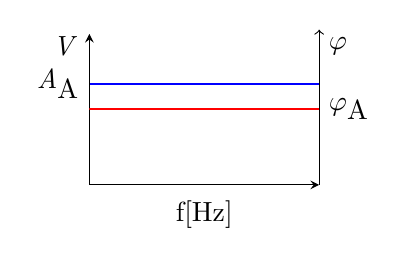
\begin{tikzpicture}[scale=1, transform shape]
    \begin{axis}[
        width=4.5cm, % Breite des Graphen
        height=3.5cm, % Höhe des Graphen
        xmin=0, xmax=10,
        ymin=0, ymax=120,
        axis lines=left,
        axis on top=true,
        domain=0:10,
        xtick=\empty,
        ytick=\empty,
        ylabel style={rotate=270, anchor=east, yshift=0.8cm}, % Position der Beschriftung oben links, horizontal
         ylabel={\it V}, % Hier die gewünschte Beschriftung einfügen
        xlabel={f[Hz]},
        clip mode=individual % Verhindert das Abschneiden von Elementen
        ]
        \addplot+[mark=none, thick, blue] coordinates {(0,80) (10,80)};
        % Adding the left-side label
        \node[anchor=east] at (axis cs:0,80) {$\mathit{A}_{\textnormal{A}}$};
    \end{axis}
    \begin{axis}[
        width=4.5cm, % Breite des Graphen
        height=3.5cm, % Höhe des Graphen
        xmin=0, xmax=10,
        ymin=-180, ymax=180,
        axis y line*=right,
        axis x line=none,
        ytick=\empty,
        ylabel={$\varphi$},
        ylabel style={rotate=270, anchor=west, yshift=0.8cm},
        clip mode=individual, % Verhindert das Abschneiden von Elementen
        after end axis/.code={
            \draw[->] (axis cs:10,180) -- (axis cs:10,190);
        }
        ]
        \addplot+[mark=none, thick, red] coordinates {(0,0) (10,0)};
        \node[anchor=west] at (axis cs:10,0) {$\varphi_{\textnormal{A}}$};
    \end{axis}
    \end{tikzpicture}
\end{center}

\vspace{1ex}
\[
\mathit{a_i} : \text{Amplitude Eingangsspannung i}
\]
\[
\mathit{\varphi_i} : \text{Phase Eingangsspannung i}
\]
\[
\mathit{A}_{A} = \sqrt{a_1^2 + a_2^2 + 2a_1a_2 \cos(\varphi_1 - \varphi_2)}
\]
\[
\mathit{\tan}(\varphi_A) = \frac{a_1 \mathit{\sin}(\varphi_1) + a_2 \mathit{\sin}(\varphi_2)}{a_1 \mathit{\cos}(\varphi_1) + a_2 \mathit{\cos}(\varphi_2)}
\]
\[
    \text{Wenn} : R_2 = R_4 = R
\]
\[
    U_{\textnormal{A}} = (1+ \frac{2R} {R_{\textnormal{g}}}) \cdot \frac{R_3} {R_2} (U_{\textnormal{E2}}-U_{\textnormal{E1}})
\]
     & 
     \textbf{Instrumentenverstärker}\newline
    Differenzverstärker mit hoher Eingangsimpedanz und hoher Gleichtaktunterdrückung  

    \\
    \hline
    \end{tabular}
\end{table}


            %\label{OPV Schaltungen Tabelle}
            %\caption{Tabelle mit ausgewählten Operationsverstärkerschaltungen}
        \end{block}
        %\label{fig:Frequenzgang OPVs}
    }	
   \b{\frametitle{Prinzip der Gegenkopplung - Lösung des Beispielproblems (3)}
    \begin{columns}
        \column[c]{0.3\textwidth}
            \begin{center}
                    \begin{circuitikz}[scale=0.8, transform shape]
        \ctikzset{tripoles/en amp/input height=-0.45,
        }
        \draw (0,0) node[en amp](E){};
        \node at ($(E) + (-1.2, 1.5)$) {\textbf{\LARGE D}}; % Label für den OPV im dritten Bild
        \draw (E.out) node[circ]{} -- ++(0.2,0) node[ocirc, right]{};
        \draw (E.-) -- ++(0, -1.3) node[circ] {} to[R, l=$R_2$] ++(2.38,0) -- ++(0,1.8);
        \draw (E.-) -- ++(0, -1.6) to[R, l_=$R_1$] ++(0, -1.2) -- ++(0,-0.2) -- ++(-0.2, 0) -- ++(0.4,0);
        \draw (E.+) node[circ]{} node[left]{};     
       
        % Spannungspfeil
        \draw[-{Triangle[width=3pt,length=4pt]}, color=spannung] ($(E.+) + (0, -0.1)$) -- ($(E.-) + (0, 0.1)$) node[midway, xshift=-32] {$U_{Diff}=0\,\text{V}$};
        \draw[-{Triangle[width=3pt,length=4pt]}, color=spannung] ($(E.out) + (0.26, -0.1)$) -- ($(E.out) + (0.26, -3.45)$) node[midway, xshift=10] {$U_A$};
        \draw[black] ($(E.out) + (0.26, -3.5)$) -- ++(-0.2, 0) -- ++(0.4,0);
        \draw[-{Triangle[width=3pt,length=4pt]}, color=spannung] (0.7,-2.1)-- ++(-1.5,0) node[midway, yshift=-8] {$U_{R2}$};
        \draw[-{Triangle[width=3pt,length=4pt]}, color=spannung] (-0.9,-2)-- ++(0,-1.5) node[midway, xshift=10] {$U_{R1}$};


        
        \node[red] at (0.9,-1.8) {\tikz \draw[red, -{Triangle[width=3pt,length=4pt]}] (0,0) -- (-0.01,0);};
        \node[above, color=red] at (0.9,-1.8)  {$I_{R2}$};

        \node[red] at ($(E.-)+(0,-1.5)$) {\tikz \draw[red, -{Triangle[width=3pt,length=4pt]}] (0,0) -- (0,-0.01);};
        \node[left, color=red] at ($(E.-)+(0,-1.4)$)  {$I_{R1}$};
      
        % Strompfeil oberhalb von R1
        %\draw[->, thick, red] (-1.19,-1) -- ++(0, -0.01);
        %\node[red] at (-1.5, -1) {$I_{R_1}$};
    \end{circuitikz}
                Finale Verstärkerschaltung mit Rückführung
                \label{fig:Verschaltung des Verstärkers2}             
            \end{center}        
        \column[c]{0.6\textwidth}
        Annahme: $U_{\textnormal{Diff}}$~=~0
        \onslide<1->{
            \begin{equation}
                U_{A} = U_{R1} + U_{R2} = U_{E} + I_{R2} \cdot R_2 
            \end{equation}}
        \onslide<2->{
            \begin{equation}
                U_{A} = U_{E} + \frac{U_{E}}{R_1} \cdot R_2 
            \end{equation}}
        \onslide<3->{
            \begin{equation}
                \frac{U_{A}}{U_{E}} = \underbrace{(1+\frac{R_2}{R_1})}_{V_{Gain}}
            \end{equation}}
        \onslide<3->{
        
        Weitere OPV-Grundschaltungen sind Skript zu finden.}
        \end{columns} 
    }
 \end{frame}

%Folie Nichtinvertierender Verstärker
\begin{frame}
    \b{
    \frametitle{Nichtinvertierender Verstärker neu}
    \begin{columns}
        \column{0.48\textwidth}
        \centering
        \begin{figure}
    \centering

    \begin{subfigure}{\linewidth}
        \centering
        \resizebox{0.6\linewidth}{!}{\begin{circuitikz}[scale=0.7, transform shape]
    \ctikzset{
         resistors/scale=0.8,              
         tripoles/en amp/height=1.4, % Höhe des OPV             
         tripoles/en amp/width=1.4,   % Breite des OPV
         tripoles/en amp/input height=-0.45
    }
    \vspace{1ex}
    \draw (2,-0.1) node[en amp] (opamp) {}
    (opamp.+) --++ (-0.5,0) node[ocirc, label=left:$U_E$] (eingang) {} 
    (opamp.out) --++ (0.5,0) node[ocirc, label=right:$U_A$] {}
    (opamp.-) -- ++(0, -1.5) to[R, l=$R_1$] ++(0, -1) node[ground] {}
    (opamp.out) node[circ] {} -- ++(0,-1.5) to[R, l=$R_2$] ++(-1.95,0) node[circ] (feedback) {};
\end{circuitikz}

}
        \caption{Schaltung eines nichtinvertierenden Verstärkers}
    \end{subfigure}

    \vspace{0.5cm} 

    \begin{subfigure}{\linewidth}
        \centering
        \resizebox{0.6\linewidth}{!}{\begin{tikzpicture}[scale=1, transform shape]
    \begin{axis}[
    width=4.5cm, % Breite des Graphen
    height=3.5cm, % Höhe des Graphen
    xmin=0, xmax=10,
    ymin=0, ymax=120,
    axis lines=left,
    axis on top=true,
    domain=0:10,
    xtick=\empty,
    ytick=\empty,
    ylabel style={rotate=270, anchor=east, yshift=1cm}, % Position der Beschriftung oben links, horizontal
     ylabel={\it V}, % Hier die gewünschte Beschriftung einfügen
    xlabel={f[Hz]},
    clip mode=individual % Verhindert das Abschneiden von Elementen
    ]
    \path[draw=none] (axis cs:-4, 0) rectangle (axis cs:16.6,120);
    
    
    \coordinate (xaxis) at (axis description cs:15.5,0); % Verwendet die relative Positionierung für x-Achse
    
    \addplot+[mark=none, thick, blue] coordinates {(0,80) (10,80)};
    % Adding the left-side label
    \node[anchor=east] at (axis cs:0,80) {$1 + \frac{R_2}{R_1}$};
    \end{axis}
    \begin{axis}[
    width=4.5cm, % Breite des Graphen
    height=3.5cm, % Höhe des Graphen
    xmin=0, xmax=10,
    ymin=-180, ymax=180,
    axis y line*=right,
    axis x line=none,
    ytick=\empty,
    ylabel={$\varphi$},
    ylabel style={rotate=270, anchor=west, yshift=0.8cm},
    clip mode=individual, % Verhindert das Abschneiden von Elementen
    after end axis/.code={
        \draw[->] (axis cs:10,180) -- (axis cs:10,190);
    }
    ]
    \addplot+[mark=none, thick, red] coordinates {(0,0) (10,0)};
    \node[anchor=west] at (axis cs:10,0) {$0^\circ$};
    \end{axis}
    \end{tikzpicture}}
        \caption{Frequenzgang eines nichtinvertierenden Verstärkers}
    \end{subfigure}

\end{figure}

        \column{0.48\textwidth}
        \begin{itemize}
            \item Gleichung:
            \[
            U_{\textnormal{A}} = \left(1+\frac{R_2}{R_1}\right) U_{\textnormal{E}}
            \]
            \item Phasengleiches Ausgangssignal
            \item Sehr hochohmiger Eingangswiderstand
            \item Niederohmiger Ausgangswiderstand
            \item Anwendungen: z.B. Impedanzwandler
        \end{itemize}
    \end{columns}
    }
\end{frame}


\begin{frame}
    \b{
    \frametitle{Nichtinvertierender Verstärker}
    \centering
    \begin{table}[ht]
    \label{tab:NichtinvertierenderVerstaerker}
    \begin{tabular}{|m{0.24\textwidth}|m{0.405\textwidth}|m{0.25\textwidth}|}
    \hline
    Schaltung & Frequenzgang und Gleichung & Erläuterung und Eigenschaften\\ % Neue Zeile mit Text
    \hline
    \vspace{0.5cm}
    \centering
    \begin{circuitikz}[scale=0.7, transform shape]
    \ctikzset{
         resistors/scale=0.8,              
         tripoles/en amp/height=1.4, % Höhe des OPV             
         tripoles/en amp/width=1.4,   % Breite des OPV
         tripoles/en amp/input height=-0.45
    }
    \vspace{1ex}
    \draw (2,-0.1) node[en amp] (opamp) {}
    (opamp.+) --++ (-0.5,0) node[ocirc, label=left:$U_E$] (eingang) {} 
    (opamp.out) --++ (0.5,0) node[ocirc, label=right:$U_A$] {}
    (opamp.-) -- ++(0, -1.5) to[R, l=$R_1$] ++(0, -1) node[ground] {}
    (opamp.out) node[circ] {} -- ++(0,-1.5) to[R, l=$R_2$] ++(-1.95,0) node[circ] (feedback) {};
\end{circuitikz}

 & \begin{tikzpicture}[scale=1, transform shape]
    \begin{axis}[
    width=4.5cm, % Breite des Graphen
    height=3.5cm, % Höhe des Graphen
    xmin=0, xmax=10,
    ymin=0, ymax=120,
    axis lines=left,
    axis on top=true,
    domain=0:10,
    xtick=\empty,
    ytick=\empty,
    ylabel style={rotate=270, anchor=east, yshift=1cm}, % Position der Beschriftung oben links, horizontal
     ylabel={\it V}, % Hier die gewünschte Beschriftung einfügen
    xlabel={f[Hz]},
    clip mode=individual % Verhindert das Abschneiden von Elementen
    ]
    \path[draw=none] (axis cs:-4, 0) rectangle (axis cs:16.6,120);
    
    
    \coordinate (xaxis) at (axis description cs:15.5,0); % Verwendet die relative Positionierung für x-Achse
    
    \addplot+[mark=none, thick, blue] coordinates {(0,80) (10,80)};
    % Adding the left-side label
    \node[anchor=east] at (axis cs:0,80) {$1 + \frac{R_2}{R_1}$};
    \end{axis}
    \begin{axis}[
    width=4.5cm, % Breite des Graphen
    height=3.5cm, % Höhe des Graphen
    xmin=0, xmax=10,
    ymin=-180, ymax=180,
    axis y line*=right,
    axis x line=none,
    ytick=\empty,
    ylabel={$\varphi$},
    ylabel style={rotate=270, anchor=west, yshift=0.8cm},
    clip mode=individual, % Verhindert das Abschneiden von Elementen
    after end axis/.code={
        \draw[->] (axis cs:10,180) -- (axis cs:10,190);
    }
    ]
    \addplot+[mark=none, thick, red] coordinates {(0,0) (10,0)};
    \node[anchor=west] at (axis cs:10,0) {$0^\circ$};
    \end{axis}
    \end{tikzpicture}
\vspace{1ex}
\[
U_{\textnormal{A}} = \left(1+\frac{R_2}{R_1}\right) U_{\textnormal{E}}
\]
    &
\begin{itemize}
    \item Phasengleiches Ausgangs-\linebreak signal
    \item Sehr hochohmiger Eingangswiderstand
    \item Niederohmiger Ausgangs-\linebreak widerstand
    \item Anwendungen: z.B. Impedanzwandler
\end{itemize} \\
    \hline
    \end{tabular}
    \end{table}
    }
\end{frame}


%Folie Invertierender Verstärker
\begin{frame}
    \b{
    \frametitle{Invertierender Verstärker}
    \centering
    \begin{table}[ht]
    \label{tab:InvertierenderVerstaerker}
    \begin{tabular}{|m{0.24\textwidth}|m{0.405\textwidth}|m{0.25\textwidth}|}
    \hline
    Schaltung & Frequenzgang und Gleichung & Erläuterung und Eigenschaften\\ % Neue Zeile mit Text
    \hline
    \vspace{0.5cm}
    \centering
    \begin{circuitikz}[scale=0.7, transform shape]
    \ctikzset{
          resistors/scale=0.8,              
          tripoles/en amp/height=1.4, % Höhe des OPV             
          tripoles/en amp/width=1.4,   % Breite des OPV
         tripoles/en amp/input height=0.45
     }
     \draw
     (0,0) node[en amp] (opamp) {}
     (opamp.-) to[R, l_=$R_1$, *-] ++(-1.2,0) to[short, o-] ++(0,0) node[left] {$U_E$}
     (opamp.+) -- ++(0,0) node[ground] {}
     (opamp.-) |- ++(0,1) to[R, l=$R_2$] ++(1.9,0) -| (opamp.out)
     (opamp.out) to[short, *-o] ++(0.2,0) node[right] {$U_{A}$};
 \end{circuitikz}
     & 
    \begin{center}
        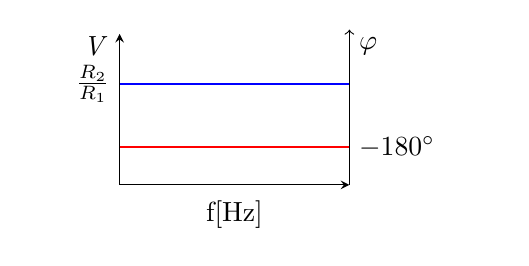
\begin{tikzpicture}[scale=1, transform shape]
    \begin{axis}[
        width=4.5cm, % Breite des Graphen
        height=3.5cm, % Höhe des Graphen
        xmin=0, xmax=10,
        ymin=0, ymax=120,
        axis lines=left,
        axis on top=true,
        domain=0:10,
        xtick=\empty,
        ytick=\empty,
        ylabel style={rotate=270, anchor=east, yshift=0.8cm},
         ylabel={\it V},
        xlabel={f[Hz]},
        clip mode=individual % Verhindert das Abschneiden von Elementen
        ]
        \path[draw=none] (axis cs:-4, 0) rectangle (axis cs:16.6,120);
    
        \addplot+[mark=none, thick, blue] coordinates {(0,80) (10,80)};
        % Adding the left-side label
        \node[anchor=east] at (axis cs:0,80) {$\frac{R_2}{R_1}$};
    \end{axis}
    \begin{axis}[
        width=4.5cm, % Breite des Graphen
        height=3.5cm, % Höhe des Graphen
        xmin=0, xmax=10,
        ymin=-180, ymax=180,
        axis y line*=right,
        axis x line=none,
        ytick=\empty,
        ylabel={$\varphi$},
        ylabel style={rotate=270, anchor=west, yshift=0.8cm},
        clip mode=individual, % Verhindert das Abschneiden von Elementen
        after end axis/.code={
            \draw[->] (axis cs:10,180) -- (axis cs:10,190);
        }
        ]
        \addplot+[mark=none, thick, red] coordinates {(0,-90) (10,-90)};
        \node[anchor=west] at (axis cs:10,-90) {$-180^\circ$};
    \end{axis}
    \end{tikzpicture}
\end{center}
\vspace{1ex}
\[
    U_{\textnormal{A}} = \frac{R_2}{R_1} U_{\textnormal{E}}
\]
    &
\begin{itemize}
    \item -180$^\circ$ Phasenverschiebung zwischen Ein- zu Ausgang
    \item $R_1$ bestimmt den Eingangswiderstand
    \item Niederohmiger Ausgangs-\linebreak widerstand
    \item Anwendungen: \linebreak z.B. Aktiver Spannungsteiler zum Messen hoher Spannungen, wenn $R_1 > R_2$
\end{itemize} \\
    \hline
    \end{tabular}
    \end{table}
    }
\end{frame}

\begin{frame}
    \b{
    \frametitle{Invertierender Verstärker neu}
    \begin{columns}
        \column{0.48\textwidth}
        \centering
        \begin{figure}
    \centering

    \begin{subfigure}{\linewidth}
        \centering
        \resizebox{0.6\linewidth}{!}{\begin{circuitikz}[scale=0.7, transform shape]
    \ctikzset{
          resistors/scale=0.8,              
          tripoles/en amp/height=1.4, % Höhe des OPV             
          tripoles/en amp/width=1.4,   % Breite des OPV
         tripoles/en amp/input height=0.45
     }
     \draw
     (0,0) node[en amp] (opamp) {}
     (opamp.-) to[R, l_=$R_1$, *-] ++(-1.2,0) to[short, o-] ++(0,0) node[left] {$U_E$}
     (opamp.+) -- ++(0,0) node[ground] {}
     (opamp.-) |- ++(0,1) to[R, l=$R_2$] ++(1.9,0) -| (opamp.out)
     (opamp.out) to[short, *-o] ++(0.2,0) node[right] {$U_{A}$};
 \end{circuitikz}}
        \caption{Schaltung eines invertierenden Verstärkers}
    \end{subfigure}

    \vspace{0.5cm} 

    \begin{subfigure}{\linewidth}
        \centering
        \resizebox{0.6\linewidth}{!}{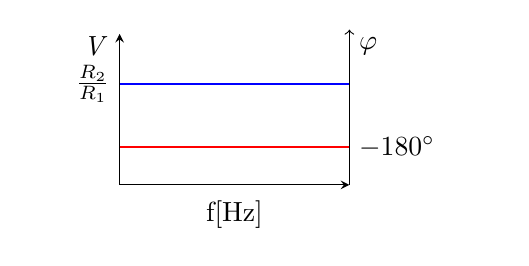
\begin{tikzpicture}[scale=1, transform shape]
    \begin{axis}[
        width=4.5cm, % Breite des Graphen
        height=3.5cm, % Höhe des Graphen
        xmin=0, xmax=10,
        ymin=0, ymax=120,
        axis lines=left,
        axis on top=true,
        domain=0:10,
        xtick=\empty,
        ytick=\empty,
        ylabel style={rotate=270, anchor=east, yshift=0.8cm},
         ylabel={\it V},
        xlabel={f[Hz]},
        clip mode=individual % Verhindert das Abschneiden von Elementen
        ]
        \path[draw=none] (axis cs:-4, 0) rectangle (axis cs:16.6,120);
    
        \addplot+[mark=none, thick, blue] coordinates {(0,80) (10,80)};
        % Adding the left-side label
        \node[anchor=east] at (axis cs:0,80) {$\frac{R_2}{R_1}$};
    \end{axis}
    \begin{axis}[
        width=4.5cm, % Breite des Graphen
        height=3.5cm, % Höhe des Graphen
        xmin=0, xmax=10,
        ymin=-180, ymax=180,
        axis y line*=right,
        axis x line=none,
        ytick=\empty,
        ylabel={$\varphi$},
        ylabel style={rotate=270, anchor=west, yshift=0.8cm},
        clip mode=individual, % Verhindert das Abschneiden von Elementen
        after end axis/.code={
            \draw[->] (axis cs:10,180) -- (axis cs:10,190);
        }
        ]
        \addplot+[mark=none, thick, red] coordinates {(0,-90) (10,-90)};
        \node[anchor=west] at (axis cs:10,-90) {$-180^\circ$};
    \end{axis}
    \end{tikzpicture}}
        \caption{Frequenzgang eines invertierenden Verstärkers}
    \end{subfigure}

\end{figure}

        \column{0.48\textwidth}
        \begin{itemize}
            \item Gleichung:
           \[
    U_{\textnormal{A}} = \frac{R_2}{R_1} U_{\textnormal{E}}
            \]
    \item -180$^\circ$ Phasenverschiebung zwischen Ein- zu Ausgang
    \item $R_1$ bestimmt den Eingangswiderstand
    \item Niederohmiger Ausgangswiderstand
    \item Anwendungen: z.B. Aktiver Spannungsteiler zum Messen hoher Spannungen, wenn $R_1 > R_2$
        \end{itemize}
    \end{columns}
    }
\end{frame}

%Folie Komparator
\begin{frame}
    \b{
    \frametitle{Komparator}
    \centering
    \begin{table}[ht]
    \label{tab:Komparator}
    \begin{tabular}{|m{0.24\textwidth}|m{0.405\textwidth}|m{0.25\textwidth}|}
    \hline
    Schaltung & Frequenzgang und Gleichung & Erläuterung und Eigenschaften\\ % Neue Zeile mit Text
    \hline
    \vspace{0.5cm}
    \centering
    \begin{circuitikz}[scale=0.7, transform shape]
    \ctikzset{
          resistors/scale=0.8,              
          tripoles/en amp/height=1.4, % Höhe des OPV             
          tripoles/en amp/width=1.4,   % Breite des OPV
         tripoles/en amp/input height=0.45
     }
     \draw
     (0,0) node[en amp] (opamp) {}
     (opamp.-)  to[short, o-] ++(0,0) node[left] {$U_{E-}$}
      (opamp.+) to[short, o-] ++(0,0) node[left] {$U_{E+}$}
     (opamp.out) to[short, -o] ++(0,0) node[right] {$U_{A}$};
 \end{circuitikz}
    & 
    \begin{center}
               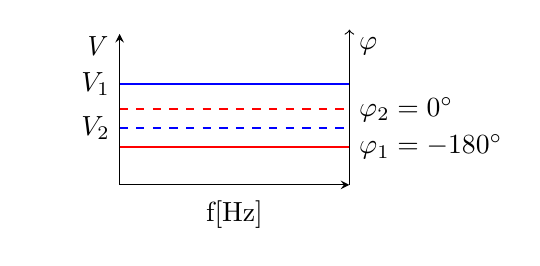
\begin{tikzpicture}[scale=1, transform shape]
    \begin{axis}[
        width=4.5cm, % Breite des Graphen
        height=3.5cm, % Höhe des Graphen
        xmin=0, xmax=10,
        ymin=0, ymax=120,
        axis lines=left,
        axis on top=true,
        domain=0:10,
        xtick=\empty,
        ytick=\empty,
        ylabel style={rotate=270, anchor=east, yshift=0.8cm},
         ylabel={\it V},
        xlabel={f[Hz]},
        clip mode=individual % Verhindert das Abschneiden von Elementen
        ]
        \path[draw=none] (axis cs:-4, 0) rectangle (axis cs:16.6,120);

        \addplot+[mark=none, thick, blue] coordinates {(0,80) (10,80)};
        \addplot+[mark=none, thick, blue, dashed] coordinates {(0,45) (10,45)};
        % Adding the left-side label
        \node[anchor=east] at (axis cs:0,80) {$V_1$};
        \node[anchor=east] at (axis cs:0,45) {$V_2$};
    \end{axis}
    \begin{axis}[
        width=4.5cm, % Breite des Graphen
        height=3.5cm, % Höhe des Graphen
        xmin=0, xmax=10,
        ymin=-180, ymax=180,
        axis y line*=right,
        axis x line=none,
        ytick=\empty,
        ylabel={$\varphi$},
        ylabel style={rotate=270, anchor=west, yshift=0.8cm},
        clip mode=individual, % Verhindert das Abschneiden von Elementen
        after end axis/.code={
            \draw[->] (axis cs:10,180) -- (axis cs:10,190);
        }
        ]
        \addplot+[mark=none, thick, red, dashed] coordinates {(0,0) (10,0)};
        \addplot+[mark=none, thick, red] coordinates {(0,-90) (10,-90)};
        \node[anchor=west] at (axis cs:10,0) {$\varphi_2 = 0^\circ$};
        \node[anchor=west] at (axis cs:10,-90) {$\varphi_1 = -180^\circ$};
    \end{axis}
    \end{tikzpicture}
\[
V_1: U_{\textnormal{E+}} > U_{\textnormal{E-}} \Rightarrow U_{\textnormal{A}} \approx +U_{\textnormal{B}}
\]
\[
V_2: U_{\textnormal{E+}} < U_{\textnormal{E-}} \Rightarrow U_{\textnormal{A}} \approx -U_{\textnormal{B}}
\]
\end{center}
    &\textbf{Komparator}\newline
    Einsatz in Zweipunktreglern und Analog-Digital-Wandlern \\
    \hline
    \end{tabular}
    \end{table}
    }
\end{frame}

\begin{frame}
    \b{
    \frametitle{Komparator neu}
    \begin{columns}
        \column{0.48\textwidth}
        \centering
        \begin{figure}
    \centering

    \begin{subfigure}{\linewidth}
        \centering
        \resizebox{0.6\linewidth}{!}{\begin{circuitikz}[scale=0.7, transform shape]
    \ctikzset{
          resistors/scale=0.8,              
          tripoles/en amp/height=1.4, % Höhe des OPV             
          tripoles/en amp/width=1.4,   % Breite des OPV
         tripoles/en amp/input height=0.45
     }
     \draw
     (0,0) node[en amp] (opamp) {}
     (opamp.-)  to[short, o-] ++(0,0) node[left] {$U_{E-}$}
      (opamp.+) to[short, o-] ++(0,0) node[left] {$U_{E+}$}
     (opamp.out) to[short, -o] ++(0,0) node[right] {$U_{A}$};
 \end{circuitikz}}
        \caption{Schaltung eines Komparators}
    \end{subfigure}

    \vspace{0.5cm} 

    \begin{subfigure}{\linewidth}
        \centering
        \resizebox{0.6\linewidth}{!}{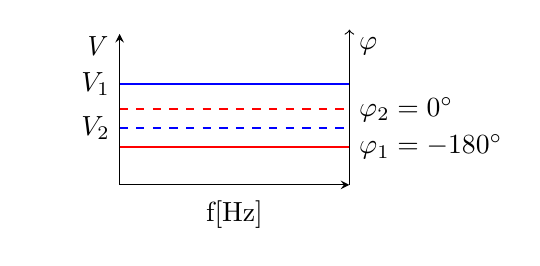
\begin{tikzpicture}[scale=1, transform shape]
    \begin{axis}[
        width=4.5cm, % Breite des Graphen
        height=3.5cm, % Höhe des Graphen
        xmin=0, xmax=10,
        ymin=0, ymax=120,
        axis lines=left,
        axis on top=true,
        domain=0:10,
        xtick=\empty,
        ytick=\empty,
        ylabel style={rotate=270, anchor=east, yshift=0.8cm},
         ylabel={\it V},
        xlabel={f[Hz]},
        clip mode=individual % Verhindert das Abschneiden von Elementen
        ]
        \path[draw=none] (axis cs:-4, 0) rectangle (axis cs:16.6,120);

        \addplot+[mark=none, thick, blue] coordinates {(0,80) (10,80)};
        \addplot+[mark=none, thick, blue, dashed] coordinates {(0,45) (10,45)};
        % Adding the left-side label
        \node[anchor=east] at (axis cs:0,80) {$V_1$};
        \node[anchor=east] at (axis cs:0,45) {$V_2$};
    \end{axis}
    \begin{axis}[
        width=4.5cm, % Breite des Graphen
        height=3.5cm, % Höhe des Graphen
        xmin=0, xmax=10,
        ymin=-180, ymax=180,
        axis y line*=right,
        axis x line=none,
        ytick=\empty,
        ylabel={$\varphi$},
        ylabel style={rotate=270, anchor=west, yshift=0.8cm},
        clip mode=individual, % Verhindert das Abschneiden von Elementen
        after end axis/.code={
            \draw[->] (axis cs:10,180) -- (axis cs:10,190);
        }
        ]
        \addplot+[mark=none, thick, red, dashed] coordinates {(0,0) (10,0)};
        \addplot+[mark=none, thick, red] coordinates {(0,-90) (10,-90)};
        \node[anchor=west] at (axis cs:10,0) {$\varphi_2 = 0^\circ$};
        \node[anchor=west] at (axis cs:10,-90) {$\varphi_1 = -180^\circ$};
    \end{axis}
    \end{tikzpicture}}
        \caption{Frequenzgang eines Komparators}
    \end{subfigure}

\end{figure}

        \column{0.48\textwidth}
        \begin{itemize}
            \item Gleichung:
          \[
V_1: U_{\textnormal{E+}} > U_{\textnormal{E-}} \Rightarrow U_{\textnormal{A}} \approx +U_{\textnormal{B}}
\]
\[
V_2: U_{\textnormal{E+}} < U_{\textnormal{E-}} \Rightarrow U_{\textnormal{A}} \approx -U_{\textnormal{B}}
\]
    \item Einsatz in Zweipunktreglern und Analog-Digital-Wandlern
        \end{itemize}
    \end{columns}
    }
\end{frame}

%Folie Summierer

\begin{frame}
    \b{
    \frametitle{Summierer}
    \centering
    \begin{table}[ht]
    \label{tab:Summierer}
    \begin{tabular}{|m{0.24\textwidth}|m{0.405\textwidth}|m{0.25\textwidth}|}
    \hline
    Schaltung & Frequenzgang und Gleichung & Erläuterung und Eigenschaften\\ % Neue Zeile mit Text
    \hline
    \vspace{0.5cm}
    \centering
    \begin{circuitikz}[scale=0.7, transform shape]
    \ctikzset{
        resistors/scale=0.8,              
        tripoles/en amp/height=1.4, % Höhe des OPV             
        tripoles/en amp/width=1.4,   % Breite des OPV
        tripoles/en amp/input height=0.45
    }
    \draw
    (0,0) node[en amp] (opamp) {}
    % R2 mit korrigiertem Strompfeil
    (opamp.-) -- ++(-0.4,0) node[circ] {} to[R, l_=$R_2$] ++(-1.5,0) node[ocirc] (R2left) {}
    % R1 mit korrigiertem Strompfeil
    (opamp.-) -- ++(-0.4,0) --++(0,1) to[R, l_=$R_1$] ++(-1.5,0) node[ocirc] (R1left) {}
    % Erdung
    (opamp.+) -- ++(0,0) node[ground] {}
    % Ausgang
    (opamp.out) to[short, *-o] ++(0,0) node[right] {$U_{A}$}
    % R3 mit Strompfeil
    (opamp.out) -- ++(0,1.5) to[R, l_=$R_3$] ++(-2,0) -- ++(0,-1.05) node[circ] {}
    % Spannungen U_E1 und U_E2 an den Knoten links von R1 und R2
    (R1left) node[left] {$U_{E1}$}
    (R2left) node[left] {$U_{E2}$};
\end{circuitikz}

    &
    \begin{center}
    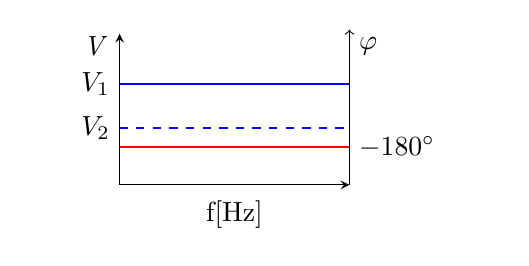
\begin{tikzpicture}[scale=1, transform shape]
    \begin{axis}[
        width=4.5cm, % Breite des Graphen
        height=3.5cm, % Höhe des Graphen
        xmin=0, xmax=10,
        ymin=0, ymax=120,
        axis lines=left,
        axis on top=true,
        domain=0:10,
        xtick=\empty,
        ytick=\empty,
        ylabel style={rotate=270, anchor=east, yshift=0.8cm},
         ylabel={\it V},
        xlabel={f[Hz]},
        clip mode=individual % Verhindert das Abschneiden von Elementen
        ]
        \addplot+[mark=none, thick, blue] coordinates {(0,80) (10,80)};
        \addplot+[mark=none, thick, blue, dashed] coordinates {(0,45) (10,45)};
    
        % Adding the left-side label
        \node[anchor=east] at (axis cs:0,80) {$V_1$};
        \node[anchor=east] at (axis cs:0,45) {$V_2$};
    \end{axis}
    \begin{axis}[
        width=4.5cm, % Breite des Graphen
        height=3.5cm, % Höhe des Graphen
        xmin=0, xmax=10,
        ymin=-180, ymax=180,
        axis y line*=right,
        axis x line=none,
        ytick=\empty,
        ylabel={$\varphi$},
        ylabel style={rotate=270, anchor=west, yshift=0.8cm},
        clip mode=individual, % Verhindert das Abschneiden von Elementen
        after end axis/.code={
            \draw[->] (axis cs:10,180) -- (axis cs:10,190);
        }
        ]
        \path[draw=none] (axis cs:-4, 0) rectangle (axis cs:16.6,120);
        \addplot+[mark=none, thick, red] coordinates {(0,-90) (10,-90)};
        \node[anchor=west] at (axis cs:10,-90) {$-180^\circ$};
    \end{axis}
    \end{tikzpicture}
\end{center}
\vspace{1ex}
\[
\begin{aligned}
    U_{\textnormal{A}} = \underbrace{\frac{R_3} {R_1}}_{V_1} \cdot U_{\textnormal{E1}} + \underbrace{\frac{R_3} {R_2}}_{V_2} \cdot U_{\textnormal{E2}}
\end{aligned}
\]
    & 
    Der Summierer basiert auf dem invertierenden Verstärker und findet Verwendung in Analogrechnern und beim Mischen von Spannungssignalen \\
    \hline
    \end{tabular}
    \end{table}
    }
\end{frame}

\begin{frame}
    \b{
    \frametitle{Summierer neu}
    \begin{columns}
        \column{0.48\textwidth}
        \centering
        \begin{figure}
    \centering

    \begin{subfigure}{\linewidth}
        \centering
        \resizebox{0.6\linewidth}{!}{\begin{circuitikz}[scale=0.7, transform shape]
    \ctikzset{
        resistors/scale=0.8,              
        tripoles/en amp/height=1.4, % Höhe des OPV             
        tripoles/en amp/width=1.4,   % Breite des OPV
        tripoles/en amp/input height=0.45
    }
    \draw
    (0,0) node[en amp] (opamp) {}
    % R2 mit korrigiertem Strompfeil
    (opamp.-) -- ++(-0.4,0) node[circ] {} to[R, l_=$R_2$] ++(-1.5,0) node[ocirc] (R2left) {}
    % R1 mit korrigiertem Strompfeil
    (opamp.-) -- ++(-0.4,0) --++(0,1) to[R, l_=$R_1$] ++(-1.5,0) node[ocirc] (R1left) {}
    % Erdung
    (opamp.+) -- ++(0,0) node[ground] {}
    % Ausgang
    (opamp.out) to[short, *-o] ++(0,0) node[right] {$U_{A}$}
    % R3 mit Strompfeil
    (opamp.out) -- ++(0,1.5) to[R, l_=$R_3$] ++(-2,0) -- ++(0,-1.05) node[circ] {}
    % Spannungen U_E1 und U_E2 an den Knoten links von R1 und R2
    (R1left) node[left] {$U_{E1}$}
    (R2left) node[left] {$U_{E2}$};
\end{circuitikz}}
        \caption{Schaltung eines Summierers}
    \end{subfigure}

    \vspace{0.5cm} 

    \begin{subfigure}{\linewidth}
        \centering
        \resizebox{0.6\linewidth}{!}{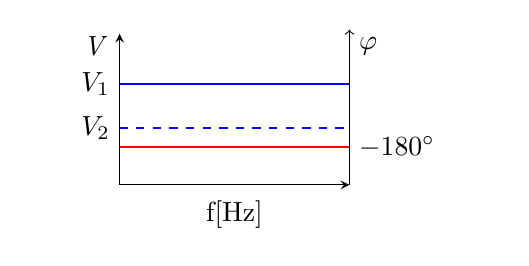
\begin{tikzpicture}[scale=1, transform shape]
    \begin{axis}[
        width=4.5cm, % Breite des Graphen
        height=3.5cm, % Höhe des Graphen
        xmin=0, xmax=10,
        ymin=0, ymax=120,
        axis lines=left,
        axis on top=true,
        domain=0:10,
        xtick=\empty,
        ytick=\empty,
        ylabel style={rotate=270, anchor=east, yshift=0.8cm},
         ylabel={\it V},
        xlabel={f[Hz]},
        clip mode=individual % Verhindert das Abschneiden von Elementen
        ]
        \addplot+[mark=none, thick, blue] coordinates {(0,80) (10,80)};
        \addplot+[mark=none, thick, blue, dashed] coordinates {(0,45) (10,45)};
    
        % Adding the left-side label
        \node[anchor=east] at (axis cs:0,80) {$V_1$};
        \node[anchor=east] at (axis cs:0,45) {$V_2$};
    \end{axis}
    \begin{axis}[
        width=4.5cm, % Breite des Graphen
        height=3.5cm, % Höhe des Graphen
        xmin=0, xmax=10,
        ymin=-180, ymax=180,
        axis y line*=right,
        axis x line=none,
        ytick=\empty,
        ylabel={$\varphi$},
        ylabel style={rotate=270, anchor=west, yshift=0.8cm},
        clip mode=individual, % Verhindert das Abschneiden von Elementen
        after end axis/.code={
            \draw[->] (axis cs:10,180) -- (axis cs:10,190);
        }
        ]
        \path[draw=none] (axis cs:-4, 0) rectangle (axis cs:16.6,120);
        \addplot+[mark=none, thick, red] coordinates {(0,-90) (10,-90)};
        \node[anchor=west] at (axis cs:10,-90) {$-180^\circ$};
    \end{axis}
    \end{tikzpicture}}
        \caption{Frequenzgang eines Summierers}
    \end{subfigure}

\end{figure}

        \column{0.48\textwidth}
        \begin{itemize}
            \item Gleichung:
          \[
U_{\textnormal{A}} = \underbrace{\frac{R_3} {R_1}}_{V_1} \cdot U_{\textnormal{E1}} + \underbrace{\frac{R_3} {R_2}}_{V_2} \cdot U_{\textnormal{E2}}
\]
    \item Der Summierer basiert auf dem invertierenden Verstärker und findet Verwendung in Analogrechnern und beim Mischen von Spannungssignalen
        \end{itemize}
    \end{columns}
    }
\end{frame}

%Folie Subtrahierer

\begin{frame}
    \b{
    \frametitle{Subtrahierer}
    \centering
    \begin{table}[ht]
    \label{tab:Subtrahierer}
    \begin{tabular}{|m{0.24\textwidth}|m{0.405\textwidth}|m{0.25\textwidth}|}
    \hline
    Schaltung & Frequenzgang und Gleichung & Erläuterung und Eigenschaften\\ % Neue Zeile mit Text
    \hline
    \vspace{0.5cm}
    \centering
    \begin{circuitikz}[scale=0.7, transform shape]
    \ctikzset{
          resistors/scale=0.8,              
          tripoles/en amp/height=1.4, % Höhe des OPV             
          tripoles/en amp/width=1.4,   % Breite des OPV
         tripoles/en amp/input height=0.45
     }
     \draw
     (0,0) node[en amp] (opamp) {}
     (opamp.-) to[R, l_=$R_1$, o-] ++(-1.2,0) to[short, o-] ++(0,0) node[left] {$U_{E1}$}
     (opamp.+) node[circ] {} to[R,  l_=$R_4$] ++(0,-1.5) node[ground] {}
     (opamp.-) node[circ] {} -- ++(0,1) to[R, l=$R_2$] ++(1.9,0) -| (opamp.out)
     (opamp.out) to[short, *-o] ++(0.2,0) node[right] {$U_{A}$}
     (opamp.+) to[R, l_=$R_3$, *-] ++(-1.2,0) to[short, o-] ++(0,0) node[left] {$U_{E2}$};
 \end{circuitikz}
      &
      \begin{center}
      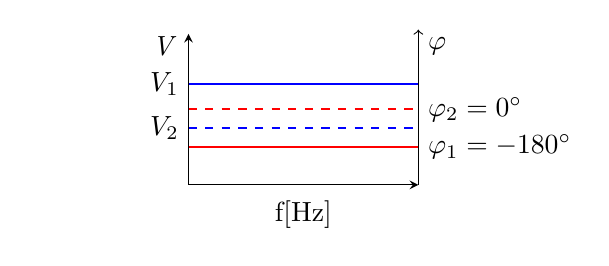
\begin{tikzpicture}[scale=1, transform shape]
    \begin{axis}[
        width=4.5cm, % Breite des Graphen
        height=3.5cm, % Höhe des Graphen
        xmin=0, xmax=10,
        ymin=0, ymax=120,
        axis lines=left,
        axis on top=true,
        domain=0:10,
        xtick=\empty,
        ytick=\empty,
        ylabel style={rotate=270, anchor=east, yshift=0.8cm},
         ylabel={\it V},
        xlabel={f[Hz]},
        clip mode=individual % Verhindert das Abschneiden von Elementen
        ]
        \addplot+[mark=none, thick, blue] coordinates {(0,80) (10,80)};
        \addplot+[mark=none, thick, blue, dashed] coordinates {(0,45) (10,45)};
        % Adding the left-side label
        \node[anchor=east] at (axis cs:0,80) {$V_1$};
        \node[anchor=east] at (axis cs:0,45) {$V_2$};
    \end{axis}
    \begin{axis}[
        width=4.5cm, % Breite des Graphen
        height=3.5cm, % Höhe des Graphen
        xmin=0, xmax=10,
        ymin=-180, ymax=180,
        axis y line*=right,
        axis x line=none,
        ytick=\empty,
        ylabel={$\varphi$},
        ylabel style={rotate=270, anchor=west, yshift=0.8cm},
        clip mode=individual, % Verhindert das Abschneiden von Elementen
        after end axis/.code={
            \draw[->] (axis cs:10,180) -- (axis cs:10,190);
        }
        ]
        \addplot+[mark=none, thick, red, dashed] coordinates {(0,0) (10,0)};
        \addplot+[mark=none, thick, red] coordinates {(0,-90) (10,-90)};
        \node[anchor=west] at (axis cs:10,0) {$\varphi_2 = 0^\circ$};
        \node[anchor=west] at (axis cs:10,-90) {$\varphi_1 = -180^\circ$};
   
   
        \path[draw=none] (axis cs:-7, 0) rectangle (axis cs:16.6,120);
   
   
   
   
    \end{axis}
    \end{tikzpicture}
 \end{center}
 \vspace{1ex}
 \[
 \begin{aligned}
    {U_A} = {U_{{\textnormal{E2}}}} \cdot \underbrace{ \frac{R_1 + R_2}{R_1} \cdot \frac{R_4}{R_3 + R_4}}_{V_2} - U_{\textnormal{E1}} \cdot \underbrace{\frac{R_2}{R_1}}_{V_1}
\end{aligned}
 \]
     &
     Wenn alle Widerstände gleich groß sind, wird die Differenz der Signale $U_{E1}$ und $U_{E2}$ gebildet, weswegen diese Schaltung als Differenzverstärker bezeichnet wird \\
    \hline
    \end{tabular}
    \end{table}
    }
\end{frame}

\begin{frame}
    \b{
    \frametitle{Subtrahierer neu}
    \begin{columns}
        \column{0.48\textwidth}
        \centering
        \begin{figure}
    \centering

    \begin{subfigure}{\linewidth}
        \centering
        \resizebox{0.6\linewidth}{!}{\begin{circuitikz}[scale=0.7, transform shape]
    \ctikzset{
          resistors/scale=0.8,              
          tripoles/en amp/height=1.4, % Höhe des OPV             
          tripoles/en amp/width=1.4,   % Breite des OPV
         tripoles/en amp/input height=0.45
     }
     \draw
     (0,0) node[en amp] (opamp) {}
     (opamp.-) to[R, l_=$R_1$, o-] ++(-1.2,0) to[short, o-] ++(0,0) node[left] {$U_{E1}$}
     (opamp.+) node[circ] {} to[R,  l_=$R_4$] ++(0,-1.5) node[ground] {}
     (opamp.-) node[circ] {} -- ++(0,1) to[R, l=$R_2$] ++(1.9,0) -| (opamp.out)
     (opamp.out) to[short, *-o] ++(0.2,0) node[right] {$U_{A}$}
     (opamp.+) to[R, l_=$R_3$, *-] ++(-1.2,0) to[short, o-] ++(0,0) node[left] {$U_{E2}$};
 \end{circuitikz}}
        \caption{Schaltung eines Subtrahierers}
    \end{subfigure}

    \vspace{0.5cm} 

    \begin{subfigure}{\linewidth}
        \centering
        \resizebox{0.6\linewidth}{!}{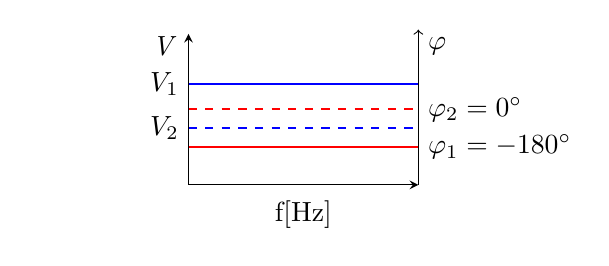
\begin{tikzpicture}[scale=1, transform shape]
    \begin{axis}[
        width=4.5cm, % Breite des Graphen
        height=3.5cm, % Höhe des Graphen
        xmin=0, xmax=10,
        ymin=0, ymax=120,
        axis lines=left,
        axis on top=true,
        domain=0:10,
        xtick=\empty,
        ytick=\empty,
        ylabel style={rotate=270, anchor=east, yshift=0.8cm},
         ylabel={\it V},
        xlabel={f[Hz]},
        clip mode=individual % Verhindert das Abschneiden von Elementen
        ]
        \addplot+[mark=none, thick, blue] coordinates {(0,80) (10,80)};
        \addplot+[mark=none, thick, blue, dashed] coordinates {(0,45) (10,45)};
        % Adding the left-side label
        \node[anchor=east] at (axis cs:0,80) {$V_1$};
        \node[anchor=east] at (axis cs:0,45) {$V_2$};
    \end{axis}
    \begin{axis}[
        width=4.5cm, % Breite des Graphen
        height=3.5cm, % Höhe des Graphen
        xmin=0, xmax=10,
        ymin=-180, ymax=180,
        axis y line*=right,
        axis x line=none,
        ytick=\empty,
        ylabel={$\varphi$},
        ylabel style={rotate=270, anchor=west, yshift=0.8cm},
        clip mode=individual, % Verhindert das Abschneiden von Elementen
        after end axis/.code={
            \draw[->] (axis cs:10,180) -- (axis cs:10,190);
        }
        ]
        \addplot+[mark=none, thick, red, dashed] coordinates {(0,0) (10,0)};
        \addplot+[mark=none, thick, red] coordinates {(0,-90) (10,-90)};
        \node[anchor=west] at (axis cs:10,0) {$\varphi_2 = 0^\circ$};
        \node[anchor=west] at (axis cs:10,-90) {$\varphi_1 = -180^\circ$};
   
   
        \path[draw=none] (axis cs:-7, 0) rectangle (axis cs:16.6,120);
   
   
   
   
    \end{axis}
    \end{tikzpicture}}
        \caption{Frequenzgang eines Subtrahierers}
    \end{subfigure}

\end{figure}

        \column{0.48\textwidth}
        \raggedleft
        \begin{itemize}
            \item Gleichung:
          \[
 {U_A} = {U_{{\textnormal{E2}}}} \cdot \underbrace{ \frac{R_1 + R_2}{R_1} \cdot \frac{R_4}{R_3 + R_4}}_{V_2} - U_{\textnormal{E1}} \cdot \underbrace{\frac{R_2}{R_1}}_{V_1}
          \]
    \item Wenn alle Widerstände gleich groß sind, wird die Differenz der Signale $U_{E1}$ und $U_{E2}$ gebildet, weswegen diese Schaltung als Differenzverstärker bezeichnet wird
        \end{itemize}
    \end{columns}
    }
\end{frame}


%Folie Integrierer

\begin{frame}
    \b{
    \frametitle{Integrierer}
    \centering
    \begin{table}[ht]
    \label{tab:Integrierer}
    \begin{tabular}{|m{0.24\textwidth}|m{0.405\textwidth}|m{0.25\textwidth}|}
    \hline
    Schaltung & Frequenzgang und Gleichung & Erläuterung und Eigenschaften\\ % Neue Zeile mit Text
    \hline
    \vspace{0.5cm}
    \centering
    \begin{circuitikz}[scale=0.7, transform shape]
    \ctikzset{
          resistors/scale=0.8,              
          tripoles/en amp/height=1.4, % Höhe des OPV             
          tripoles/en amp/width=1.4,   % Breite des OPV
         capacitors/scale=0.5,
         tripoles/en amp/input height=0.45
     }
     \vspace{1ex}
     \draw (2,0) node[en amp] (opamp) {}
     (opamp.+) --++ (-0.5,0) node[ground] {} 
     (opamp.out) --++ (0.2,0) node[ocirc, label=right:$U_A$] {}
     (opamp.-) -- ++(0, 0) to[R, l_=$R_1$] ++(-1.2, 0) node[ocirc, label=left:$U_E$] {}
     
     (opamp.out) node[circ] {} -- ++(0,1.5) to[C, l_=$C_1$, *-] ++(-1.9,0) node[circ]{}
     (opamp.out) node[circ] {} -- ++(0,2.8) to[R, l_=$R_2$] ++(-1.9,0) -- ++(0, -2.35) node[circ] {};
     \end{circuitikz}
     & 
     \begin{center}
    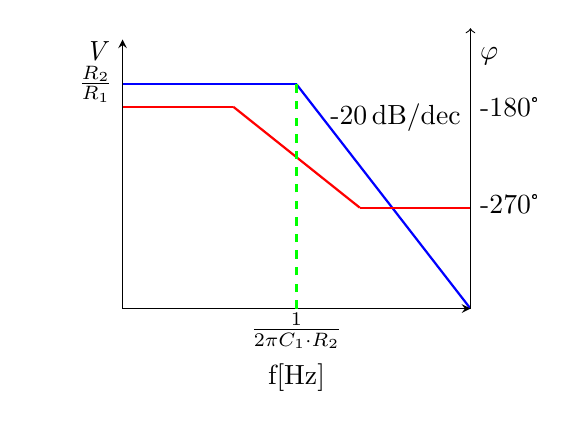
\begin{tikzpicture}[scale=1, transform shape]
    \begin{axis}[
       width=6cm, % Breite des Graphen
       height=5cm, % Höhe des Graphen
        xmin=0, xmax=11,
        ymin=0, ymax=1.2,
        axis lines=center,
        axis on top=true,
        domain=0:10,
        xtick=\empty,
        ytick=\empty,
        ylabel style={xshift=-0.6cm, yshift=0.1cm },
       ylabel={\it V},
       xlabel style={yshift=-0.4cm },
        xlabel={f[Hz]},
        clip mode=individual, % Verhindert das Abschneiden von Elementen
        xlabel style={at={(axis description cs:0.5,-0.05)},anchor=north}
        ]

        \path[draw=none] (axis cs:-3, 0) rectangle (axis cs:13,1);



        \addplot+[mark=none, thick, blue] coordinates {(0,1) (5.5,1)};
        \addplot+[mark=none, thick, blue] coordinates {(5.5,1) (11,0)};
        \node[anchor=east] at (axis cs:0,1) {$\frac{R_2}{R_1}$};
       \node[anchor=east] at (axis cs:11,0.85) {-20\,\text{dB/dec}};
    \end{axis}
    
    \begin{axis}[
       width=6cm, % Breite des Graphen
       height=5cm, % Höhe des Graphen
       xmin=0, xmax=11,
       ymin=0, ymax=240, 
       axis y line*=right,
       axis x line=none,
       ylabel={$\varphi$},
       ylabel style={rotate=270, anchor=west, yshift=1.5cm},
       xtick=\empty,
       ytick=\empty,
       clip mode=individual, % Verhindert das Abschneiden von Elementen
       after end axis/.code={
           \draw[->] (axis cs:11,240) -- (axis cs:11,250);
       }
        ]
        \addplot+[mark=none, thick, red] coordinates {(0,180) (3.5,180)};
        \addplot+[mark=none, thick, red] coordinates {(3.5,180) (7.5,90)};
        \addplot+[mark=none, thick, red] coordinates {(7.5,90) (11,90)};
        \addplot+[mark=none,dashed, thick, green] coordinates {(5.5,0) (5.5,200)};
        \node[] at (axis cs:5.5,-20) {$\frac{1}{2 \pi C_1 \cdot R_2}$};
        \node[anchor=west] at (axis cs:11,180) {-180°};
        \node[anchor=west] at (axis cs:11,93) {-270°};
    \end{axis}
    \end{tikzpicture}
     \[
     U_A(t) = - \frac{R_2}{R_1} U_{\textnormal{E}}(t) - \int_0^t \frac{U_{\textnormal{E}}(t)}{R_1 C_1} \, dt
     \]
     \end{center} 
     &
    \begin{itemize}
        \item Nimmt eine Integration des Eingangssignals vor
        \item Wird als aktives Tiefpassfilter verwendet
    \end{itemize} \\
    \hline
    \end{tabular}
    \end{table}
    }
\end{frame}

\begin{frame}
    \b{
    \frametitle{Integrierer neu}
    \begin{columns}
        \column{0.48\textwidth}
        \centering
        \begin{figure}
    \centering

    \begin{subfigure}{\linewidth}
        \centering
        \resizebox{0.6\linewidth}{!}{\begin{circuitikz}[scale=0.7, transform shape]
    \ctikzset{
          resistors/scale=0.8,              
          tripoles/en amp/height=1.4, % Höhe des OPV             
          tripoles/en amp/width=1.4,   % Breite des OPV
         capacitors/scale=0.5,
         tripoles/en amp/input height=0.45
     }
     \vspace{1ex}
     \draw (2,0) node[en amp] (opamp) {}
     (opamp.+) --++ (-0.5,0) node[ground] {} 
     (opamp.out) --++ (0.2,0) node[ocirc, label=right:$U_A$] {}
     (opamp.-) -- ++(0, 0) to[R, l_=$R_1$] ++(-1.2, 0) node[ocirc, label=left:$U_E$] {}
     
     (opamp.out) node[circ] {} -- ++(0,1.5) to[C, l_=$C_1$, *-] ++(-1.9,0) node[circ]{}
     (opamp.out) node[circ] {} -- ++(0,2.8) to[R, l_=$R_2$] ++(-1.9,0) -- ++(0, -2.35) node[circ] {};
     \end{circuitikz}}
        \caption{Schaltung eines Integrierers}
    \end{subfigure}

    \vspace{0.5cm} 

    \begin{subfigure}{\linewidth}
        \centering
        \resizebox{0.6\linewidth}{!}{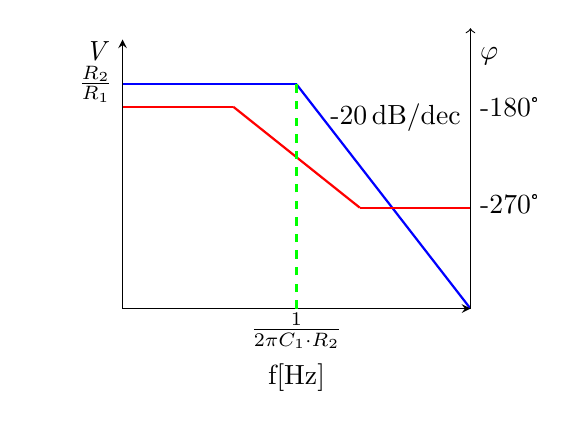
\begin{tikzpicture}[scale=1, transform shape]
    \begin{axis}[
       width=6cm, % Breite des Graphen
       height=5cm, % Höhe des Graphen
        xmin=0, xmax=11,
        ymin=0, ymax=1.2,
        axis lines=center,
        axis on top=true,
        domain=0:10,
        xtick=\empty,
        ytick=\empty,
        ylabel style={xshift=-0.6cm, yshift=0.1cm },
       ylabel={\it V},
       xlabel style={yshift=-0.4cm },
        xlabel={f[Hz]},
        clip mode=individual, % Verhindert das Abschneiden von Elementen
        xlabel style={at={(axis description cs:0.5,-0.05)},anchor=north}
        ]

        \path[draw=none] (axis cs:-3, 0) rectangle (axis cs:13,1);



        \addplot+[mark=none, thick, blue] coordinates {(0,1) (5.5,1)};
        \addplot+[mark=none, thick, blue] coordinates {(5.5,1) (11,0)};
        \node[anchor=east] at (axis cs:0,1) {$\frac{R_2}{R_1}$};
       \node[anchor=east] at (axis cs:11,0.85) {-20\,\text{dB/dec}};
    \end{axis}
    
    \begin{axis}[
       width=6cm, % Breite des Graphen
       height=5cm, % Höhe des Graphen
       xmin=0, xmax=11,
       ymin=0, ymax=240, 
       axis y line*=right,
       axis x line=none,
       ylabel={$\varphi$},
       ylabel style={rotate=270, anchor=west, yshift=1.5cm},
       xtick=\empty,
       ytick=\empty,
       clip mode=individual, % Verhindert das Abschneiden von Elementen
       after end axis/.code={
           \draw[->] (axis cs:11,240) -- (axis cs:11,250);
       }
        ]
        \addplot+[mark=none, thick, red] coordinates {(0,180) (3.5,180)};
        \addplot+[mark=none, thick, red] coordinates {(3.5,180) (7.5,90)};
        \addplot+[mark=none, thick, red] coordinates {(7.5,90) (11,90)};
        \addplot+[mark=none,dashed, thick, green] coordinates {(5.5,0) (5.5,200)};
        \node[] at (axis cs:5.5,-20) {$\frac{1}{2 \pi C_1 \cdot R_2}$};
        \node[anchor=west] at (axis cs:11,180) {-180°};
        \node[anchor=west] at (axis cs:11,93) {-270°};
    \end{axis}
    \end{tikzpicture}}
        \caption{Frequenzgang eines Integrierers}
    \end{subfigure}

\end{figure}

        \column{0.48\textwidth}
        \raggedleft
        \begin{itemize}
            \item Gleichung:
           \[
     U_A(t) = - \frac{R_2}{R_1} U_{\textnormal{E}}(t) - \int_0^t \frac{U_{\textnormal{E}}(t)}{R_1 C_1} \, dt
     \]
        \item Nimmt eine Integration des Eingangssignals vor
        \item Wird als aktives Tiefpassfilter verwendet     
    \end{itemize}
    \end{columns}
    }
\end{frame}

%Folie Differenzierer

\begin{frame}
    \b{
    \frametitle{Differenzierer}
    \centering
    \begin{table}[ht]
    \label{tab:Differenzierer}
    \begin{tabular}{|m{0.24\textwidth}|m{0.405\textwidth}|m{0.25\textwidth}|}
    \hline
    Schaltung & Frequenzgang und Gleichung & Erläuterung und Eigenschaften\\ % Neue Zeile mit Text
    \hline
    \vspace{0.5cm}
    \centering
    \begin{circuitikz}[scale=0.7, transform shape]
    \ctikzset{
          resistors/scale=0.8,              
          tripoles/en amp/height=1.4, % Höhe des OPV             
          tripoles/en amp/width=1.4,   % Breite des OPV
         capacitors/scale=0.5,
         tripoles/en amp/input height=0.45
     }
     \draw (2,0) node[en amp] (opamp) {}
     (opamp.+) --++ (-0.5,0) node[ground] {} 
     (opamp.out) --++ (0.2,0) node[ocirc, label=right:$U_A$] {}
     (opamp.-) -- ++(0, 0) to[C, l_=$C_2$] ++(-0.5, 0) to[R, l_=$R_1$] ++(-1.2,0) node[ocirc, label=left:$U_E$] {}
     (opamp.out) node[circ] {} -- ++(0,1.5) to[C, l_=$C_1$, *-] ++(-1.9,0) node[circ]{}
     (opamp.out) node[circ] {} -- ++(0,2.8) to[R, l_=$R_2$] ++(-1.9,0) -- ++(0, -2.35) node[circ] {};
  
 \end{circuitikz}
    &
    \begin{center}
    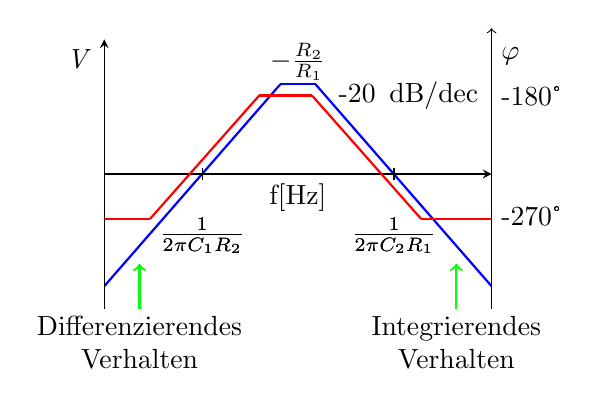
\begin{tikzpicture}[scale=1, transform shape]
    \begin{axis}[
        width=6.5cm, % Breite des Graphen
        height=5cm, % Höhe des Graphen
        xmin=0, xmax=11,
        ymin=-1.2, ymax=1.2,
        axis lines=center,
        axis on top=true,
        domain=0:10,
        clip mode=individual, % Verhindert das Abschneiden von Elementen
        xtick=\empty,
        ytick=\empty,
        ylabel style={xshift=-0.6cm},
        ylabel={\it V},
        xlabel={f[Hz]},
        xlabel style={at={(axis description cs:0.5,0.5)},anchor=north}
        ]
        \path[draw=none] (axis cs:-2, 0) rectangle (axis cs:13,1); \path[draw=none] (axis cs:-2, 0) rectangle (axis cs:13,1);


        \addplot+[mark=none, thick, blue] coordinates {(0,-1) (5,0.8)};
        \addplot+[mark=none, thick, blue] coordinates {(5,0.8) (6,0.8)};
        \addplot+[mark=none, thick, blue] coordinates {(6,0.8) (11,-1)};
        \node[anchor=north] at (axis cs:5.5,1.25) {$-\frac{R_2}{R_1}$};
        \addplot+[only marks, mark=|, black] coordinates {(2.78,0)} node[anchor=south] at (axis cs:2.78,-0.8) {$\frac{1}{2 \pi C_1 R_2}$};
        \addplot+[only marks, mark=|, black] coordinates {(8.23,0)} node[anchor=south] at (axis cs:8.23,-0.8) {$\frac{1}{2\pi C_2 R_1}$};
        \node[anchor=east] at (axis cs:10.9,0.7) {-20\, \text{dB/dec}};
        \addplot+[only marks, mark=|, black] coordinates {(2.78,0)} node[anchor=south] at (axis cs:2.78,-0.8) {$\frac{1}{2 \pi C_1 R_2}$};
        \addplot+[only marks, mark=|, black] coordinates {(8.23,0)} node[anchor=south] at (axis cs:8.23,-0.8) {$\frac{1}{2\pi C_2 R_1}$};
        \draw[->, thick, green] (axis cs:1,-1.2) -- (axis cs:1,-0.8);
        \node[align=center, black] at (axis cs:1,-1.5) {Differenzierendes\\ Verhalten};
        
        \draw[->, thick, green] (axis cs:10,-1.2) -- (axis cs:10,-0.8);
        \node[align=center, black] at (axis cs:10,-1.5) {Integrierendes\\ Verhalten};
        
    \end{axis}
    
    \begin{axis}[
        width=6.5cm, % Breite des Graphen
        height=5cm, % Höhe des Graphen
        xmin=0, xmax=11,
        ymin=0, ymax=240, 
        axis y line*=right,
        axis x line=none,
        ylabel={$\varphi$},
        ylabel style={rotate=270, anchor=west, yshift=1.5cm},
        xtick=\empty,
        ytick=\empty,
        clip mode=individual, % Verhindert das Abschneiden von Elementen
        after end axis/.code={
            \draw[->] (axis cs:11,240) -- (axis cs:11,250);
        }
        ]
        \addplot+[mark=none, thick, red] coordinates {(0,80) (1.3,80)};
        \addplot+[mark=none, thick, red] coordinates {(1.3,80) (4.4,190)};
        \addplot+[mark=none, thick, red] coordinates {(4.4,190) (5.9,190)};
        \addplot+[mark=none, thick, red] coordinates {(5.9,190) (9,80)};
        \addplot+[mark=none, thick, red] coordinates {(9,80) (11,80)};
        \node[anchor=west] at (axis cs:11,82.5) {-270°};
        \node[anchor=west] at (axis cs:11,190) {-180°};
       
    \end{axis}

    
    \end{tikzpicture}
    \begin{multline*}
        U_A = - \frac{R_2}{R_1} U_{\textnormal{E}}(t) \\
        - \int_0^t \frac{1}{R_1 C_1} U_{\textnormal{E}}(t) \, dt 
        - R_2 C_2\frac{dU_{\textnormal{E}}(t)}{dt}
    \end{multline*}
    \end{center} 
    & 
    \textbf{Differenzierer}\newline
    \begin{itemize}
        \item Nimmt eine Integration des Eingangssignals vor
        \item Wird als aktives Hochpassfilter verwendet (zeigt in der Realität meist Bandpassverhalten, wie hier dargestellt)
    \end{itemize} \\
    \hline
    \end{tabular}
    \end{table}
    }
\end{frame}

\begin{frame}
    \b{
    \frametitle{Differenzierer neu}
    \begin{columns}
        \column{0.48\textwidth}
        \centering
        \begin{figure}
    \centering

    \begin{subfigure}{\linewidth}
        \centering
        \resizebox{0.6\linewidth}{!}{\begin{circuitikz}[scale=0.7, transform shape]
    \ctikzset{
          resistors/scale=0.8,              
          tripoles/en amp/height=1.4, % Höhe des OPV             
          tripoles/en amp/width=1.4,   % Breite des OPV
         capacitors/scale=0.5,
         tripoles/en amp/input height=0.45
     }
     \draw (2,0) node[en amp] (opamp) {}
     (opamp.+) --++ (-0.5,0) node[ground] {} 
     (opamp.out) --++ (0.2,0) node[ocirc, label=right:$U_A$] {}
     (opamp.-) -- ++(0, 0) to[C, l_=$C_2$] ++(-0.5, 0) to[R, l_=$R_1$] ++(-1.2,0) node[ocirc, label=left:$U_E$] {}
     (opamp.out) node[circ] {} -- ++(0,1.5) to[C, l_=$C_1$, *-] ++(-1.9,0) node[circ]{}
     (opamp.out) node[circ] {} -- ++(0,2.8) to[R, l_=$R_2$] ++(-1.9,0) -- ++(0, -2.35) node[circ] {};
  
 \end{circuitikz}}
        \caption{Schaltung eines Differenzierers}
    \end{subfigure}

    \vspace{0.5cm} 

    \begin{subfigure}{\linewidth}
        \centering
        \resizebox{0.6\linewidth}{!}{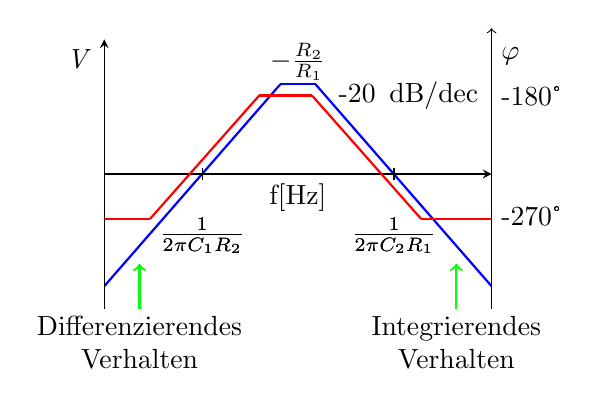
\begin{tikzpicture}[scale=1, transform shape]
    \begin{axis}[
        width=6.5cm, % Breite des Graphen
        height=5cm, % Höhe des Graphen
        xmin=0, xmax=11,
        ymin=-1.2, ymax=1.2,
        axis lines=center,
        axis on top=true,
        domain=0:10,
        clip mode=individual, % Verhindert das Abschneiden von Elementen
        xtick=\empty,
        ytick=\empty,
        ylabel style={xshift=-0.6cm},
        ylabel={\it V},
        xlabel={f[Hz]},
        xlabel style={at={(axis description cs:0.5,0.5)},anchor=north}
        ]
        \path[draw=none] (axis cs:-2, 0) rectangle (axis cs:13,1); \path[draw=none] (axis cs:-2, 0) rectangle (axis cs:13,1);


        \addplot+[mark=none, thick, blue] coordinates {(0,-1) (5,0.8)};
        \addplot+[mark=none, thick, blue] coordinates {(5,0.8) (6,0.8)};
        \addplot+[mark=none, thick, blue] coordinates {(6,0.8) (11,-1)};
        \node[anchor=north] at (axis cs:5.5,1.25) {$-\frac{R_2}{R_1}$};
        \addplot+[only marks, mark=|, black] coordinates {(2.78,0)} node[anchor=south] at (axis cs:2.78,-0.8) {$\frac{1}{2 \pi C_1 R_2}$};
        \addplot+[only marks, mark=|, black] coordinates {(8.23,0)} node[anchor=south] at (axis cs:8.23,-0.8) {$\frac{1}{2\pi C_2 R_1}$};
        \node[anchor=east] at (axis cs:10.9,0.7) {-20\, \text{dB/dec}};
        \addplot+[only marks, mark=|, black] coordinates {(2.78,0)} node[anchor=south] at (axis cs:2.78,-0.8) {$\frac{1}{2 \pi C_1 R_2}$};
        \addplot+[only marks, mark=|, black] coordinates {(8.23,0)} node[anchor=south] at (axis cs:8.23,-0.8) {$\frac{1}{2\pi C_2 R_1}$};
        \draw[->, thick, green] (axis cs:1,-1.2) -- (axis cs:1,-0.8);
        \node[align=center, black] at (axis cs:1,-1.5) {Differenzierendes\\ Verhalten};
        
        \draw[->, thick, green] (axis cs:10,-1.2) -- (axis cs:10,-0.8);
        \node[align=center, black] at (axis cs:10,-1.5) {Integrierendes\\ Verhalten};
        
    \end{axis}
    
    \begin{axis}[
        width=6.5cm, % Breite des Graphen
        height=5cm, % Höhe des Graphen
        xmin=0, xmax=11,
        ymin=0, ymax=240, 
        axis y line*=right,
        axis x line=none,
        ylabel={$\varphi$},
        ylabel style={rotate=270, anchor=west, yshift=1.5cm},
        xtick=\empty,
        ytick=\empty,
        clip mode=individual, % Verhindert das Abschneiden von Elementen
        after end axis/.code={
            \draw[->] (axis cs:11,240) -- (axis cs:11,250);
        }
        ]
        \addplot+[mark=none, thick, red] coordinates {(0,80) (1.3,80)};
        \addplot+[mark=none, thick, red] coordinates {(1.3,80) (4.4,190)};
        \addplot+[mark=none, thick, red] coordinates {(4.4,190) (5.9,190)};
        \addplot+[mark=none, thick, red] coordinates {(5.9,190) (9,80)};
        \addplot+[mark=none, thick, red] coordinates {(9,80) (11,80)};
        \node[anchor=west] at (axis cs:11,82.5) {-270°};
        \node[anchor=west] at (axis cs:11,190) {-180°};
       
    \end{axis}

    
    \end{tikzpicture}}
        \caption{Frequenzgang eines Differenzierers}
    \end{subfigure}

\end{figure}

        \column{0.48\textwidth}
        \raggedleft
        \begin{itemize}
            \item Gleichung:
          \[
U_{\textnormal{A}}(t) = 
- \frac{R_2}{R_1} \, U_{\textnormal{E}}(t)
- \int_0^t \frac{1}{R_1 C_1} \, U_{\textnormal{E}}(\tau) \, d\tau
- R_2 C_2 \, \frac{dU_{\textnormal{E}}}{dt}(t)
\]

        \item Nimmt eine Integration des Eingangssignals vor
        \item Wird als aktives Hochpassfilter verwendet (zeigt in der Realität meist Bandpassverhalten, wie hier dargestellt)  
    \end{itemize}
    \end{columns}
    }
\end{frame}

%Folie Logarithmierer

\begin{frame}
    \b{
    \frametitle{Logarithmierer}
    \centering
    \begin{table}[ht]
    \label{tab:Logarithmierer}
    \begin{tabular}{|m{0.24\textwidth}|m{0.405\textwidth}|m{0.25\textwidth}|}
    \hline
    Schaltung & Frequenzgang und Gleichung & Erläuterung und Eigenschaften\\ % Neue Zeile mit Text
    \hline
    \vspace{0.5cm}
    \centering
    \begin{circuitikz}[scale=0.7, transform shape]
    \ctikzset{
          resistors/scale=0.8,              
          tripoles/en amp/height=1.4, % Höhe des OPV             
          tripoles/en amp/width=1.4,   % Breite des OPV
         diodes/scale=0.8,
         tripoles/en amp/input height=0.45
     }
     \draw
     (0,0) node[en amp] (opamp) {}
     (opamp.-) to[R, l_=$R_1$, *-] ++(-1.2,0) to[short, o-] ++(0,0) node[left] {$U_E$}
     (opamp.+) -- ++(0,0) node[ground] {}
     (opamp.-) |- ++(0,1.5) to[D, l^=$D_1$] ++(2,0) -| (opamp.out)
     (opamp.out) to[short, *-o] ++(0.2,0) node[right] {$U_{A}$};
 \end{circuitikz}
    &
    \begin{center}
    \[
    U_{\textnormal{A}} =-U_{\textnormal{T}}\cdot \ln{\left(\frac{U_{\textnormal{E}}}{R_1\cdot I_S}\right)}
    \]
        \[
            U_{\textnormal{T}} = \frac{k_{\textnormal{B}} \cdot T}{e}
            \]
            
            \(e = \text{Elementarladung}\)
            
            \(k_{\textnormal{B}} = \text{Boltzmannkonstante}\)
            
            \(I_{\textnormal{s}} = \text{Sperrstrom der Diode}\)
    \end{center} 
    & 
    Bildet den natürlichen Logarithmus des Eingangssignals \\
    \hline
    \end{tabular}
    \end{table}
    }
\end{frame}

\begin{frame}
    \b{
    \frametitle{Logarithmierer neu}
    \begin{columns}
        \column{0.48\textwidth}
        \centering
        \begin{figure}
    \centering
        \begin{circuitikz}[scale=0.7, transform shape]
    \ctikzset{
          resistors/scale=0.8,              
          tripoles/en amp/height=1.4, % Höhe des OPV             
          tripoles/en amp/width=1.4,   % Breite des OPV
         diodes/scale=0.8,
         tripoles/en amp/input height=0.45
     }
     \draw
     (0,0) node[en amp] (opamp) {}
     (opamp.-) to[R, l_=$R_1$, *-] ++(-1.2,0) to[short, o-] ++(0,0) node[left] {$U_E$}
     (opamp.+) -- ++(0,0) node[ground] {}
     (opamp.-) |- ++(0,1.5) to[D, l^=$D_1$] ++(2,0) -| (opamp.out)
     (opamp.out) to[short, *-o] ++(0.2,0) node[right] {$U_{A}$};
 \end{circuitikz}
        \caption{Schaltung eines Logarithmierers}

\end{figure}

        \column{0.48\textwidth}
        \raggedleft
        \begin{itemize}
            \item Gleichung:
           \[
    U_{\textnormal{A}} =-U_{\textnormal{T}}\cdot \ln{\left(\frac{U_{\textnormal{E}}}{R_1\cdot I_S}\right)}
    \]
        \[
            U_{\textnormal{T}} = \frac{k_{\textnormal{B}} \cdot T}{e}
            \]
            
            \(e = \text{Elementarladung}\)
            
            \(k_{\textnormal{B}} = \text{Boltzmannkonstante}\)
            
            \(I_{\textnormal{s}} = \text{Sperrstrom der Diode}\)
        \item Bildet den natürlichen Logarithmus des Eingangssignals
    \end{itemize}
    \end{columns}
    }
\end{frame}

%Folie Potenzierer

\begin{frame}
    \b{
        \frametitle{Potenzierer}
    \centering
    \begin{table}[ht]
    \label{tab:Potenzierer}
    \begin{tabular}{|m{0.24\textwidth}|m{0.405\textwidth}|m{0.25\textwidth}|}
    \hline
    Schaltung & Frequenzgang und Gleichung & Erläuterung und Eigenschaften\\ % Neue Zeile mit Text
    \hline
    \vspace{0.5cm}
    \centering
    \begin{circuitikz}[scale=0.7, transform shape]
    \ctikzset{
          resistors/scale=0.8,              
          tripoles/en amp/height=1.4, % Höhe des OPV            
          tripoles/en amp/width=1.4,   % Breite des OPV
         diodes/scale=0.8,
         tripoles/en amp/input height=0.45
     }
     \draw
     (0,0) node[en amp] (opamp) {}
     (opamp.-) to[D, l_=$D_1$, invert, *-] ++(-1.2,0) to[short, o-] ++(0,0) node[left] {$U_E$}
     (opamp.+) -- ++(0,0) node[ground] {}
     (opamp.-) |- ++(0,1.5) to[R, l^=$R_1$] ++(2,0) -| (opamp.out)
     (opamp.out) to[short, *-o] ++(0.2,0) node[right] {$U_{A}$};
 \end{circuitikz}
    &
    \begin{center}
    \[
    U_{\textnormal{A}} =-R_1\cdot I_{\textnormal{S}} \cdot e^{\frac{U_{\textnormal{E}}}{U_{\textnormal{T}}}}
    \]
    \end{center} 
    & 
    Besitzt einen e-funktionalen Zusammenhang zwischen Ein- und Ausgangsspannung \\
    \hline
    \end{tabular}
    \end{table}
    }
\end{frame}

\begin{frame}
    \b{
    \frametitle{Potenzierer neu}
    \begin{columns}
        \column{0.48\textwidth}
        \centering
        \begin{figure}
        \centering
        {\begin{circuitikz}[scale=0.7, transform shape]
    \ctikzset{
          resistors/scale=0.8,              
          tripoles/en amp/height=1.4, % Höhe des OPV            
          tripoles/en amp/width=1.4,   % Breite des OPV
         diodes/scale=0.8,
         tripoles/en amp/input height=0.45
     }
     \draw
     (0,0) node[en amp] (opamp) {}
     (opamp.-) to[D, l_=$D_1$, invert, *-] ++(-1.2,0) to[short, o-] ++(0,0) node[left] {$U_E$}
     (opamp.+) -- ++(0,0) node[ground] {}
     (opamp.-) |- ++(0,1.5) to[R, l^=$R_1$] ++(2,0) -| (opamp.out)
     (opamp.out) to[short, *-o] ++(0.2,0) node[right] {$U_{A}$};
 \end{circuitikz}}
        \caption{Schaltung eines Potenzierers}

\end{figure}

        \column{0.48\textwidth}
        \raggedleft
        \begin{itemize}
            \item Gleichung:
           \[
    U_{\textnormal{A}} =-R_1\cdot I_{\textnormal{S}} \cdot e^{\frac{U_{\textnormal{E}}}{U_{\textnormal{T}}}}
    \]
        \item Besitzt einen e-funktionalen Zusammenhang zwischen Ein- und Ausgangsspannung
    \end{itemize}
    \end{columns}
    }
\end{frame}

%Folie Insutrmentenverstärker 

\begin{frame}
    \b{
        \frametitle{Instrumentenverstärker}
    \centering
    \begin{table}[ht]
    \label{tab:Instrumentenverstaerker}
    \begin{tabular}{|m{0.24\textwidth}|m{0.405\textwidth}|m{0.25\textwidth}|}
    \hline
    Schaltung & Frequenzgang und Gleichung & Erläuterung und Eigenschaften\\ % Neue Zeile mit Text
    \hline
    \vspace{0.5cm}
    \centering
    \begin{circuitikz}[scale=0.6, transform shape]
    \ctikzset{
         resistors/scale=0.8,              
         tripoles/en amp/height=1.4, % Höhe des OPV             
         tripoles/en amp/width=1.4   % Breite des OPV
    }
    \draw 
    % Erster OPV mit input height=-0.45
    (2,-4.5) node[en amp, noinv input down] (opamp1) {}
    (opamp1.+) --++ (-0.5,0) node[ocirc, label=left:$U_{E2}$] (eingang1) {};
    
   \draw (2,0) node[en amp, noinv input up] (opamp2) {}
    (opamp2.+) --++ (-0.5,0) node[ocirc, label=left:$U_{E1}$] (eingang2) {}
    (opamp1.-)  to[R=$R_g$] (opamp2.-);

   % Dritter OPV mit angepasstem Eingangsabstand
    \ctikzset{tripoles/en amp/input height=0.55} % Anpassung nur für diesen OPV
    \draw (6,-2.25) node[en amp] (opamp3) {}
    (opamp3.-) -- ++(-0.5,0) to[R=$R_1$] ++(-1.5,0) to[R=$R_2$] ++(-2,0) node[circ]{}
    (opamp3.+) -- ++(-0.5,0) to[R=$R_3$] ++(-1.5,0) to[R=$R_4$] ++(-2,0) node[circ]{}
    (opamp2.out) -- ++(0,-1.72) node[circ]{}
    (opamp1.out) -- ++(0,1.72) node[circ]{}
    (opamp3.out) node[circ, label=below:{$U_A$}]{} -- ++(0, 2) to[R=$R_5$] ++(-2,0) -- ++(0, -1.45)node[circ]{};

\end{circuitikz}
     &
         \begin{center}
   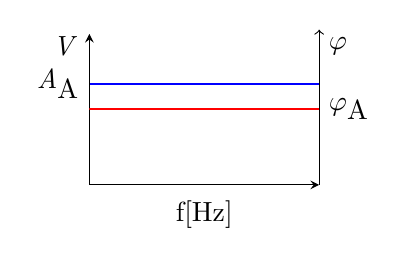
\begin{tikzpicture}[scale=1, transform shape]
    \begin{axis}[
        width=4.5cm, % Breite des Graphen
        height=3.5cm, % Höhe des Graphen
        xmin=0, xmax=10,
        ymin=0, ymax=120,
        axis lines=left,
        axis on top=true,
        domain=0:10,
        xtick=\empty,
        ytick=\empty,
        ylabel style={rotate=270, anchor=east, yshift=0.8cm}, % Position der Beschriftung oben links, horizontal
         ylabel={\it V}, % Hier die gewünschte Beschriftung einfügen
        xlabel={f[Hz]},
        clip mode=individual % Verhindert das Abschneiden von Elementen
        ]
        \addplot+[mark=none, thick, blue] coordinates {(0,80) (10,80)};
        % Adding the left-side label
        \node[anchor=east] at (axis cs:0,80) {$\mathit{A}_{\textnormal{A}}$};
    \end{axis}
    \begin{axis}[
        width=4.5cm, % Breite des Graphen
        height=3.5cm, % Höhe des Graphen
        xmin=0, xmax=10,
        ymin=-180, ymax=180,
        axis y line*=right,
        axis x line=none,
        ytick=\empty,
        ylabel={$\varphi$},
        ylabel style={rotate=270, anchor=west, yshift=0.8cm},
        clip mode=individual, % Verhindert das Abschneiden von Elementen
        after end axis/.code={
            \draw[->] (axis cs:10,180) -- (axis cs:10,190);
        }
        ]
        \addplot+[mark=none, thick, red] coordinates {(0,0) (10,0)};
        \node[anchor=west] at (axis cs:10,0) {$\varphi_{\textnormal{A}}$};
    \end{axis}
    \end{tikzpicture}
\end{center}

\vspace{1ex}
\[
\mathit{a_i} : \text{Amplitude Eingangsspannung i}
\]
\[
\mathit{\varphi_i} : \text{Phase Eingangsspannung i}
\]
\[
\mathit{A}_{A} = \sqrt{a_1^2 + a_2^2 + 2a_1a_2 \cos(\varphi_1 - \varphi_2)}
\]
\[
\mathit{\tan}(\varphi_A) = \frac{a_1 \mathit{\sin}(\varphi_1) + a_2 \mathit{\sin}(\varphi_2)}{a_1 \mathit{\cos}(\varphi_1) + a_2 \mathit{\cos}(\varphi_2)}
\]
\[
    \text{Wenn} : R_2 = R_4 = R
\]
\[
    U_{\textnormal{A}} = (1+ \frac{2R} {R_{\textnormal{g}}}) \cdot \frac{R_3} {R_2} (U_{\textnormal{E2}}-U_{\textnormal{E1}})
\]
     & 
    Differenzverstärker mit hoher Eingangsimpedanz und hoher Gleichtaktunterdrückung  
 \\
    \hline
    \end{tabular}
    \end{table}
    }
\end{frame}

\begin{frame}
    \b{
    \frametitle{Instrumentenverstärker neu}
    \begin{columns}
        \column{0.48\textwidth}
        \centering
        \begin{figure}
    \centering

    \begin{subfigure}{\linewidth}
        \centering
        \resizebox{0.6\linewidth}{!}{\begin{circuitikz}[scale=0.6, transform shape]
    \ctikzset{
         resistors/scale=0.8,              
         tripoles/en amp/height=1.4, % Höhe des OPV             
         tripoles/en amp/width=1.4   % Breite des OPV
    }
    \draw 
    % Erster OPV mit input height=-0.45
    (2,-4.5) node[en amp, noinv input down] (opamp1) {}
    (opamp1.+) --++ (-0.5,0) node[ocirc, label=left:$U_{E2}$] (eingang1) {};
    
   \draw (2,0) node[en amp, noinv input up] (opamp2) {}
    (opamp2.+) --++ (-0.5,0) node[ocirc, label=left:$U_{E1}$] (eingang2) {}
    (opamp1.-)  to[R=$R_g$] (opamp2.-);

   % Dritter OPV mit angepasstem Eingangsabstand
    \ctikzset{tripoles/en amp/input height=0.55} % Anpassung nur für diesen OPV
    \draw (6,-2.25) node[en amp] (opamp3) {}
    (opamp3.-) -- ++(-0.5,0) to[R=$R_1$] ++(-1.5,0) to[R=$R_2$] ++(-2,0) node[circ]{}
    (opamp3.+) -- ++(-0.5,0) to[R=$R_3$] ++(-1.5,0) to[R=$R_4$] ++(-2,0) node[circ]{}
    (opamp2.out) -- ++(0,-1.72) node[circ]{}
    (opamp1.out) -- ++(0,1.72) node[circ]{}
    (opamp3.out) node[circ, label=below:{$U_A$}]{} -- ++(0, 2) to[R=$R_5$] ++(-2,0) -- ++(0, -1.45)node[circ]{};

\end{circuitikz}}
        \caption{Schaltung eines Instrumentenverstärkers}
    \end{subfigure}

    \vspace{0.5cm} 

    \begin{subfigure}{\linewidth}
        \centering
        \resizebox{0.6\linewidth}{!}{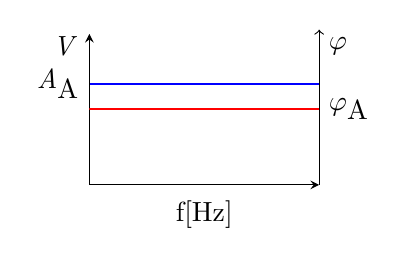
\begin{tikzpicture}[scale=1, transform shape]
    \begin{axis}[
        width=4.5cm, % Breite des Graphen
        height=3.5cm, % Höhe des Graphen
        xmin=0, xmax=10,
        ymin=0, ymax=120,
        axis lines=left,
        axis on top=true,
        domain=0:10,
        xtick=\empty,
        ytick=\empty,
        ylabel style={rotate=270, anchor=east, yshift=0.8cm}, % Position der Beschriftung oben links, horizontal
         ylabel={\it V}, % Hier die gewünschte Beschriftung einfügen
        xlabel={f[Hz]},
        clip mode=individual % Verhindert das Abschneiden von Elementen
        ]
        \addplot+[mark=none, thick, blue] coordinates {(0,80) (10,80)};
        % Adding the left-side label
        \node[anchor=east] at (axis cs:0,80) {$\mathit{A}_{\textnormal{A}}$};
    \end{axis}
    \begin{axis}[
        width=4.5cm, % Breite des Graphen
        height=3.5cm, % Höhe des Graphen
        xmin=0, xmax=10,
        ymin=-180, ymax=180,
        axis y line*=right,
        axis x line=none,
        ytick=\empty,
        ylabel={$\varphi$},
        ylabel style={rotate=270, anchor=west, yshift=0.8cm},
        clip mode=individual, % Verhindert das Abschneiden von Elementen
        after end axis/.code={
            \draw[->] (axis cs:10,180) -- (axis cs:10,190);
        }
        ]
        \addplot+[mark=none, thick, red] coordinates {(0,0) (10,0)};
        \node[anchor=west] at (axis cs:10,0) {$\varphi_{\textnormal{A}}$};
    \end{axis}
    \end{tikzpicture}}
        \caption{Frequenzgang eines Instrumentenverstärkers}
    \end{subfigure}

\end{figure}

        \column{0.48\textwidth}
        \raggedleft
        \begin{itemize}
            \item Gleichung:
         \[
\mathit{a_i} : \text{Amplitude Eingangsspannung i}
\]
\[
\mathit{\varphi_i} : \text{Phase Eingangsspannung i}
\]
\[
\mathit{A}_{A} = \sqrt{a_1^2 + a_2^2 + 2a_1a_2 \cos(\varphi_1 - \varphi_2)}
\]
\[
\mathit{\tan}(\varphi_A) = \frac{a_1 \mathit{\sin}(\varphi_1) + a_2 \mathit{\sin}(\varphi_2)}{a_1 \mathit{\cos}(\varphi_1) + a_2 \mathit{\cos}(\varphi_2)}
\]
\[
    \text{Wenn} : R_2 = R_4 = R
\]
\[
    U_{\textnormal{A}} = (1+ \frac{2R} {R_{\textnormal{g}}}) \cdot \frac{R_3} {R_2} (U_{\textnormal{E2}}-U_{\textnormal{E1}})
\]
        \item Differenzverstärker mit hoher Eingangsimpedanz und hoher Gleichtaktunterdrückung    
    \end{itemize}
    \end{columns}
    }
\end{frame}


%Folie Insutrmentenverstärker 

\begin{frame}
    \b{
        \frametitle{Impedanzwandler}
    \centering
    \begin{table}[ht]
    \label{tab:Impedanzwandler}
    \begin{tabular}{|m{0.24\textwidth}|m{0.405\textwidth}|m{0.25\textwidth}|}
    \hline
    Schaltung & Frequenzgang und Gleichung & Erläuterung und Eigenschaften\\ % Neue Zeile mit Text
    \hline
    \vspace{0.5cm}
    \centering
    \scalebox{0.45}{\begin{circuitikz}
    \ctikzset{tripoles/en amp/input height=0.45}
\draw (0,0)node[en amp, en amp text A](E){}
    (E.out)
    (E.-)
    (E.+);
\draw (E.-) -- (-1.5,0.5) -- (-1.5,2) -- (2,2) to[short,-*] (2,0);
\draw (E.out) to[short, -o] ( 3,0);
\draw (3,-2) to[short, o-o] (-3,-2);
\draw (0,-2)node[ground]{};
\draw (E.+) to[short,-o] (-3,-0.5);


\draw (-3,-0.5) to[open,v>, name=ue] (-3,-2);
\draw (3,0) to[open,v>, name=ua] (3,-2);
\varrmore{ua}{$U_\mathrm{A}$};
\varrmore{ue}{$U_\mathrm{E}$};
\end{circuitikz}}
     &

\vspace{1ex}
Ausgangsspannung $U_\mathrm{A}$ folgt der Eingangsspannung $U_\mathrm{E}$ \newline
Verstärkung $V = \frac{U_\mathrm{A}}{U_\mathrm{E}} = 1$ 

     & 
    
     Auch Spannungsfolger genannt \newline
     Hoher Eingangswiderstand durch Operationsverstärker \newline
     Typische Anwendung: Sensoren

 \\
    \hline
    \end{tabular}
    \end{table}
    }
\end{frame}

\begin{frame}
    \b{
    \frametitle{Impedanzwandler neu}
    \begin{columns}
        \column{0.48\textwidth}
        \centering
        \begin{figure}
        \centering
        \begin{circuitikz}
    \ctikzset{tripoles/en amp/input height=0.45}
\draw (0,0)node[en amp, en amp text A](E){}
    (E.out)
    (E.-)
    (E.+);
\draw (E.-) -- (-1.5,0.5) -- (-1.5,2) -- (2,2) to[short,-*] (2,0);
\draw (E.out) to[short, -o] ( 3,0);
\draw (3,-2) to[short, o-o] (-3,-2);
\draw (0,-2)node[ground]{};
\draw (E.+) to[short,-o] (-3,-0.5);


\draw (-3,-0.5) to[open,v>, name=ue] (-3,-2);
\draw (3,0) to[open,v>, name=ua] (3,-2);
\varrmore{ua}{$U_\mathrm{A}$};
\varrmore{ue}{$U_\mathrm{E}$};
\end{circuitikz}
        \caption{Schaltung eines Impedanzwandlers}

\end{figure}

        \column{0.48\textwidth}
        \centering
        \begin{itemize}
        \item Ausgangsspannung $U_\mathrm{A}$ folgt der Eingangsspannung $U_\mathrm{E}$ 
        \item Verstärkung $V = \frac{U_\mathrm{A}}{U_\mathrm{E}} = 1$ 
        \item Auch Spannungsfolger genannt
        \item Hoher Eingangswiderstand durch Operationsverstärker
        \item Typische Anwendung: Sensoren
    \end{itemize}
    \end{columns}
    }
\end{frame}